% Options for packages loaded elsewhere
\PassOptionsToPackage{unicode}{hyperref}
\PassOptionsToPackage{hyphens}{url}
\PassOptionsToPackage{dvipsnames,svgnames*,x11names*}{xcolor}
%
\documentclass[
  10pt,
]{article}
\usepackage{lmodern}
\usepackage{amssymb,amsmath}
\usepackage{ifxetex,ifluatex}
\ifnum 0\ifxetex 1\fi\ifluatex 1\fi=0 % if pdftex
  \usepackage[T1]{fontenc}
  \usepackage[utf8]{inputenc}
  \usepackage{textcomp} % provide euro and other symbols
\else % if luatex or xetex
  \usepackage{unicode-math}
  \defaultfontfeatures{Scale=MatchLowercase}
  \defaultfontfeatures[\rmfamily]{Ligatures=TeX,Scale=1}
\fi
% Use upquote if available, for straight quotes in verbatim environments
\IfFileExists{upquote.sty}{\usepackage{upquote}}{}
\IfFileExists{microtype.sty}{% use microtype if available
  \usepackage[]{microtype}
  \UseMicrotypeSet[protrusion]{basicmath} % disable protrusion for tt fonts
}{}
\makeatletter
\@ifundefined{KOMAClassName}{% if non-KOMA class
  \IfFileExists{parskip.sty}{%
    \usepackage{parskip}
  }{% else
    \setlength{\parindent}{0pt}
    \setlength{\parskip}{6pt plus 2pt minus 1pt}}
}{% if KOMA class
  \KOMAoptions{parskip=half}}
\makeatother
\usepackage{xcolor}
\IfFileExists{xurl.sty}{\usepackage{xurl}}{} % add URL line breaks if available
\IfFileExists{bookmark.sty}{\usepackage{bookmark}}{\usepackage{hyperref}}
\hypersetup{
  pdftitle={Modeling Food and Housing Insecurity at UTEP},
  pdfauthor={George E. Quaye; John Koomson; Willliam O. Agyapong},
  colorlinks=true,
  linkcolor=blue,
  filecolor=Maroon,
  citecolor=Blue,
  urlcolor=Blue,
  pdfcreator={LaTeX via pandoc}}
\urlstyle{same} % disable monospaced font for URLs
\usepackage[margin = 0.8in]{geometry}
\usepackage{longtable,booktabs}
% Correct order of tables after \paragraph or \subparagraph
\usepackage{etoolbox}
\makeatletter
\patchcmd\longtable{\par}{\if@noskipsec\mbox{}\fi\par}{}{}
\makeatother
% Allow footnotes in longtable head/foot
\IfFileExists{footnotehyper.sty}{\usepackage{footnotehyper}}{\usepackage{footnote}}
\makesavenoteenv{longtable}
\usepackage{graphicx,grffile}
\makeatletter
\def\maxwidth{\ifdim\Gin@nat@width>\linewidth\linewidth\else\Gin@nat@width\fi}
\def\maxheight{\ifdim\Gin@nat@height>\textheight\textheight\else\Gin@nat@height\fi}
\makeatother
% Scale images if necessary, so that they will not overflow the page
% margins by default, and it is still possible to overwrite the defaults
% using explicit options in \includegraphics[width, height, ...]{}
\setkeys{Gin}{width=\maxwidth,height=\maxheight,keepaspectratio}
% Set default figure placement to htbp
\makeatletter
\def\fps@figure{htbp}
\makeatother
\setlength{\emergencystretch}{3em} % prevent overfull lines
\providecommand{\tightlist}{%
  \setlength{\itemsep}{0pt}\setlength{\parskip}{0pt}}
\setcounter{secnumdepth}{5}
\usepackage{float}
\usepackage{setspace}
\doublespacing
\usepackage{bm}
\usepackage{amsmath}
\usepackage{amssymb}
\usepackage{amsfonts}
\usepackage{amsthm}
\usepackage{fancyhdr}
\pagestyle{fancy}
\fancyhf{}
\rhead{George Quaye, John Koomson, William Agyapong}
\lhead{Phase II Report - DS 6335}
\cfoot{\thepage}
\usepackage{algorithm}
\usepackage[noend]{algpseudocode}
\usepackage{booktabs}
\usepackage{longtable}
\usepackage{array}
\usepackage{multirow}
\usepackage{wrapfig}
\usepackage{float}
\usepackage{colortbl}
\usepackage{pdflscape}
\usepackage{tabu}
\usepackage{threeparttable}
\usepackage{threeparttablex}
\usepackage[normalem]{ulem}
\usepackage{makecell}
\usepackage{xcolor}

\title{Modeling Food and Housing Insecurity at UTEP}
\usepackage{etoolbox}
\makeatletter
\providecommand{\subtitle}[1]{% add subtitle to \maketitle
  \apptocmd{\@title}{\par {\large #1 \par}}{}{}
}
\makeatother
\subtitle{Phase II Report}
\author{George E. Quaye \and John Koomson \and Willliam O. Agyapong}
\date{\center University of Texas, El Paso (UTEP)\center \center Department of Mathematical Sciences \center}

\begin{document}
\maketitle

{
\hypersetup{linkcolor=}
\setcounter{tocdepth}{4}
\tableofcontents
}
\hypertarget{discussion}{%
\section{Discussion}\label{discussion}}

It was clearly noticed from our analysis that given each best model, predicting whether one is food insecure or housing insecure for the six responses, the factors or variables such as total income, transportation reliability, type of residence, specifically residence off-campus with family, whether or not one is the head of the household and the number of dependents on the person were part of the major contributing factors. However, we made a weird observation, which is among the subgroups at risk for food insecurity factors, total income for people earning more than \$100,000 were occurring in all four responses, which analytical and socially does not make sense. In general, total income being an underlying factor for both food insecurity and housing insecurity, clearly suggests that the income on which students live for their livelihood appears not to be enough.

Considering the factors affecting housing insecurity responses, permanent house address and spending the night elsewhere, both were found to be associated with transport reliability, household head, the college one comes from, and whether the person is living alone, and total income as the most important variables among others. That is to say, the chances of one being housing insecure rely on one's total income, one being a household head with more dependents, and how reliable their transportation is with regards to one's income and expenditure. Also considering which subgroups or populations are at risk of being housing insecure, factors including having a residence off-campus with family, coming from either a college of education or college of science, and having a very reliable transportation mode. Specifically, it appears that if a student belongs to the college of science or college of education and stays off-campus with the family coupled with having a reliable common mode of transportation is at risk at a point in time of housing insecurity should that person is being deprived of such benefits.

Furthermore, the Logistics model and support vector machine dominated as the best model for modeling and predicting food insecurity response variables. The topmost factor predicting food insecurity from all four modeled response was the total income of the person, mode of transport, and its reliability, whether one know of any homeless student, household head, the number of dependents, and finally whether one is employed or not. Suggesting that one becoming food insecure depends on one income, numbers of dependents, and more as depicted by the model graphs. Identifying which person or persons are at risk of food being insecure was characterized by people living off-campus with family, someone been black or African American, and enrolled as a junior and having more than four dependents. Specifically, a Black American enrolled as a junior living with a family off campus with more than four dependents is a high risk of being food insecure.

Our initial preferred model or models were selected based on the evaluation metrics accuracy, misclassification, fbeta, and the area under the curve (AUC) from each response variable table obtained. That is, a model with the least misclassification, higher accuracy, an fbeta score approaching one, and a higher AUC. However, our initial preferred model or models may or may not be sufficient enough to make a predictive decision because they may involve irregularities. As an improvement to phase one of our modelings, we employed post hoc predictive modeling to ascertain the initial preferred models. Specifically, we employed the ensemble analysis model to train our obtained several related but different analytical models (SVM, LDA, etc..) and then synthesized the results into a single score or spread in order to improve the accuracy of prediction. We made use of this idea of the ensemble method because a single model based on a data sample can have biases, high variability, or outright inaccuracies that affect the reliability of its analytical findings. By combining these different models we can reduce the effects of those limitations and provide better predictive information from the learning model. After the best predictive models are chosen a plot of variables of importance were obtained to determine which variables are most significant in predicting a given response variable, and also to answer the research question of which subgroup are at risk of a given food and house insecurity response.

\hypertarget{analysis-and-results}{%
\section{Analysis and Results}\label{analysis-and-results}}

\hypertarget{exploratory-data-analysis}{%
\subsection{Exploratory Data Analysis}\label{exploratory-data-analysis}}

\hypertarget{summary-statistics}{%
\subsubsection{Summary Statistics}\label{summary-statistics}}

Table 2 shows how the various variables used throughout the analysis are distributed across their respective levels, after data cleaning, accounting for double counting in multiple response instances, and collapsing levels where we considered appropriate. Missing values are denoted by \textbf{NA}, so variables with the additional \textbf{NA} level are those with missing observations.

\begingroup\fontsize{9}{11}\selectfont

\begin{longtable}[t]{llccc}
\caption{\label{tab:summary-stats} A summary of variables of interest}\\
\toprule
Variable Name & Levels & Coded As & Obervations & Percentage\\
\midrule
\endfirsthead
\caption[]{\label{tab:summary-stats} A summary of variables of interest \textit{(continued)}}\\
\toprule
Variable Name & Levels & Coded As & Obervations & Percentage\\
\midrule
\endhead

\endfoot
\bottomrule
\endlastfoot
\cellcolor{gray!6}{enrollment} & \cellcolor{gray!6}{Full Time} & \cellcolor{gray!6}{1} & \cellcolor{gray!6}{4325} & \cellcolor{gray!6}{83.57\%}\\
\cellcolor{gray!6}{} & \cellcolor{gray!6}{Part Time} & \cellcolor{gray!6}{2} & \cellcolor{gray!6}{850} & \cellcolor{gray!6}{16.43\%}\\
employment & Full Time & 1 & 968 & 18.71\%\\
 & Part Time & 2 & 2006 & 38.76\%\\
 & No & 3 & 2201 & 42.53\%\\
\cellcolor{gray!6}{employment\_type} & \cellcolor{gray!6}{On-Campus} & \cellcolor{gray!6}{1} & \cellcolor{gray!6}{491} & \cellcolor{gray!6}{16.51\%}\\
\cellcolor{gray!6}{} & \cellcolor{gray!6}{Off-Campus} & \cellcolor{gray!6}{2} & \cellcolor{gray!6}{2483} & \cellcolor{gray!6}{83.49\%}\\
weekly\_work\_hrs & 19 hours or less & 1 & 1337 & 44.96\%\\
 & More than 19 hours & 2 & 1637 & 55.04\%\\
\cellcolor{gray!6}{ethnicity} & \cellcolor{gray!6}{Hispanic} & \cellcolor{gray!6}{1} & \cellcolor{gray!6}{4462} & \cellcolor{gray!6}{86.22\%}\\
\cellcolor{gray!6}{} & \cellcolor{gray!6}{Asian} & \cellcolor{gray!6}{2} & \cellcolor{gray!6}{115} & \cellcolor{gray!6}{2.22\%}\\
\cellcolor{gray!6}{} & \cellcolor{gray!6}{Black/African American} & \cellcolor{gray!6}{3} & \cellcolor{gray!6}{135} & \cellcolor{gray!6}{2.61\%}\\
\cellcolor{gray!6}{} & \cellcolor{gray!6}{White/Caucasian} & \cellcolor{gray!6}{4} & \cellcolor{gray!6}{291} & \cellcolor{gray!6}{5.62\%}\\
\cellcolor{gray!6}{} & \cellcolor{gray!6}{Other} & \cellcolor{gray!6}{5} & \cellcolor{gray!6}{172} & \cellcolor{gray!6}{3.32\%}\\
gender & Female & 1 & 3508 & 67.79\%\\
 & Male & 2 & 1583 & 30.59\%\\
 & Non-binary/Non-conforming & 3 & 62 & 1.20\%\\
 & NA &  & 22 & 0.43\%\\
\cellcolor{gray!6}{total\_income} & \cellcolor{gray!6}{< 10,000} & \cellcolor{gray!6}{1} & \cellcolor{gray!6}{851} & \cellcolor{gray!6}{16.44\%}\\
\cellcolor{gray!6}{} & \cellcolor{gray!6}{10,000-19,999} & \cellcolor{gray!6}{2} & \cellcolor{gray!6}{862} & \cellcolor{gray!6}{16.66\%}\\
\cellcolor{gray!6}{} & \cellcolor{gray!6}{20,000-29,999} & \cellcolor{gray!6}{3} & \cellcolor{gray!6}{806} & \cellcolor{gray!6}{15.57\%}\\
\cellcolor{gray!6}{} & \cellcolor{gray!6}{30,000-39,000} & \cellcolor{gray!6}{4} & \cellcolor{gray!6}{649} & \cellcolor{gray!6}{12.54\%}\\
\cellcolor{gray!6}{} & \cellcolor{gray!6}{40,000-49,999} & \cellcolor{gray!6}{5} & \cellcolor{gray!6}{538} & \cellcolor{gray!6}{10.40\%}\\
\cellcolor{gray!6}{} & \cellcolor{gray!6}{50,000-69,999} & \cellcolor{gray!6}{6} & \cellcolor{gray!6}{651} & \cellcolor{gray!6}{12.58\%}\\
\cellcolor{gray!6}{} & \cellcolor{gray!6}{70,000-99,999} & \cellcolor{gray!6}{7} & \cellcolor{gray!6}{494} & \cellcolor{gray!6}{9.55\%}\\
\cellcolor{gray!6}{} & \cellcolor{gray!6}{>=100,000} & \cellcolor{gray!6}{8} & \cellcolor{gray!6}{324} & \cellcolor{gray!6}{6.26\%}\\
academic\_level & Freshman & 1 & 709 & 13.70\%\\
 & Sophomore & 2 & 739 & 14.28\%\\
 & Junior & 3 & 1275 & 24.64\%\\
 & Senior & 4 & 1628 & 31.46\%\\
 & Masters & 5 & 559 & 10.80\%\\
 & Doctoral/Professional & 6 & 265 & 5.12\%\\
\cellcolor{gray!6}{college/school} & \cellcolor{gray!6}{Business} & \cellcolor{gray!6}{1} & \cellcolor{gray!6}{573} & \cellcolor{gray!6}{11.07\%}\\
\cellcolor{gray!6}{} & \cellcolor{gray!6}{Education} & \cellcolor{gray!6}{2} & \cellcolor{gray!6}{484} & \cellcolor{gray!6}{9.35\%}\\
\cellcolor{gray!6}{} & \cellcolor{gray!6}{Engineering} & \cellcolor{gray!6}{3} & \cellcolor{gray!6}{838} & \cellcolor{gray!6}{16.19\%}\\
\cellcolor{gray!6}{} & \cellcolor{gray!6}{Health Sciences} & \cellcolor{gray!6}{4} & \cellcolor{gray!6}{577} & \cellcolor{gray!6}{11.15\%}\\
\cellcolor{gray!6}{} & \cellcolor{gray!6}{Liberal Arts} & \cellcolor{gray!6}{5} & \cellcolor{gray!6}{1274} & \cellcolor{gray!6}{24.62\%}\\
\cellcolor{gray!6}{} & \cellcolor{gray!6}{Science} & \cellcolor{gray!6}{6} & \cellcolor{gray!6}{822} & \cellcolor{gray!6}{15.88\%}\\
\cellcolor{gray!6}{} & \cellcolor{gray!6}{Nursing} & \cellcolor{gray!6}{7} & \cellcolor{gray!6}{423} & \cellcolor{gray!6}{8.17\%}\\
\cellcolor{gray!6}{} & \cellcolor{gray!6}{Pharmacy} & \cellcolor{gray!6}{8} & \cellcolor{gray!6}{41} & \cellcolor{gray!6}{0.79\%}\\
\cellcolor{gray!6}{} & \cellcolor{gray!6}{Other} & \cellcolor{gray!6}{9} & \cellcolor{gray!6}{55} & \cellcolor{gray!6}{1.06\%}\\
\cellcolor{gray!6}{} & \cellcolor{gray!6}{More than one} & \cellcolor{gray!6}{10} & \cellcolor{gray!6}{88} & \cellcolor{gray!6}{1.70\%}\\
mode\_transport & Car (alone) & 1 & 3359 & 64.91\%\\
 & Car (someone drives) \& Carpool & 2 & 805 & 15.56\%\\
 & Bus/Public transport & 3 & 398 & 7.69\%\\
 & Bike, Trolley, or Walk & 4 & 179 & 3.46\%\\
 & Other & 5 & 125 & 2.42\%\\
 & Not applicable & 6 & 309 & 5.97\%\\
\cellcolor{gray!6}{transport\_reliability} & \cellcolor{gray!6}{Not reliable at all} & \cellcolor{gray!6}{1} & \cellcolor{gray!6}{92} & \cellcolor{gray!6}{1.89\%}\\
\cellcolor{gray!6}{} & \cellcolor{gray!6}{Somewhat reliable} & \cellcolor{gray!6}{2} & \cellcolor{gray!6}{429} & \cellcolor{gray!6}{8.82\%}\\
\cellcolor{gray!6}{} & \cellcolor{gray!6}{Fairly reliable} & \cellcolor{gray!6}{3} & \cellcolor{gray!6}{1628} & \cellcolor{gray!6}{33.46\%}\\
\cellcolor{gray!6}{} & \cellcolor{gray!6}{Very reliable} & \cellcolor{gray!6}{4} & \cellcolor{gray!6}{2717} & \cellcolor{gray!6}{55.84\%}\\
living\_alone & Yes & 1 & 441 & 8.52\%\\
 & No & 2 & 4734 & 91.48\%\\
\cellcolor{gray!6}{dependents} & \cellcolor{gray!6}{0} & \cellcolor{gray!6}{1} & \cellcolor{gray!6}{3802} & \cellcolor{gray!6}{73.47\%}\\
\cellcolor{gray!6}{} & \cellcolor{gray!6}{1} & \cellcolor{gray!6}{2} & \cellcolor{gray!6}{367} & \cellcolor{gray!6}{7.09\%}\\
\cellcolor{gray!6}{} & \cellcolor{gray!6}{2 - 3} & \cellcolor{gray!6}{3} & \cellcolor{gray!6}{448} & \cellcolor{gray!6}{8.66\%}\\
\cellcolor{gray!6}{} & \cellcolor{gray!6}{4 or more} & \cellcolor{gray!6}{4} & \cellcolor{gray!6}{98} & \cellcolor{gray!6}{1.89\%}\\
\cellcolor{gray!6}{} & \cellcolor{gray!6}{NA} & \cellcolor{gray!6}{} & \cellcolor{gray!6}{460} & \cellcolor{gray!6}{8.89\%}\\
household\_head & Yes & 1 & 1155 & 22.32\%\\
 & No & 2 & 3964 & 76.60\%\\
 & NA &  & 56 & 1.08\%\\
\cellcolor{gray!6}{residence} & \cellcolor{gray!6}{On-Campus} & \cellcolor{gray!6}{1} & \cellcolor{gray!6}{133} & \cellcolor{gray!6}{2.57\%}\\
\cellcolor{gray!6}{} & \cellcolor{gray!6}{Off-Campus with family} & \cellcolor{gray!6}{2} & \cellcolor{gray!6}{4093} & \cellcolor{gray!6}{79.09\%}\\
\cellcolor{gray!6}{} & \cellcolor{gray!6}{Off-Campus not with family} & \cellcolor{gray!6}{3} & \cellcolor{gray!6}{821} & \cellcolor{gray!6}{15.86\%}\\
\cellcolor{gray!6}{} & \cellcolor{gray!6}{Other} & \cellcolor{gray!6}{4} & \cellcolor{gray!6}{48} & \cellcolor{gray!6}{0.93\%}\\
\cellcolor{gray!6}{} & \cellcolor{gray!6}{NA} & \cellcolor{gray!6}{} & \cellcolor{gray!6}{80} & \cellcolor{gray!6}{\vphantom{1} 1.55\%}\\
permanent\_address & Yes & 1 & 4830 & 93.33\%\\
 & No & 2 & 265 & 5.12\%\\
 & NA &  & 80 & 1.55\%\\
\cellcolor{gray!6}{spent\_night\_elsewhere} & \cellcolor{gray!6}{Rarely} & \cellcolor{gray!6}{1} & \cellcolor{gray!6}{138} & \cellcolor{gray!6}{52.08\%}\\
\cellcolor{gray!6}{} & \cellcolor{gray!6}{Sometimes} & \cellcolor{gray!6}{2} & \cellcolor{gray!6}{83} & \cellcolor{gray!6}{31.32\%}\\
\cellcolor{gray!6}{} & \cellcolor{gray!6}{Often} & \cellcolor{gray!6}{3} & \cellcolor{gray!6}{33} & \cellcolor{gray!6}{12.45\%}\\
\cellcolor{gray!6}{} & \cellcolor{gray!6}{NA} & \cellcolor{gray!6}{} & \cellcolor{gray!6}{11} & \cellcolor{gray!6}{4.15\%}\\
know\_homeless\_student & Yes & 1 & 965 & 18.65\%\\
 & No & 2 & 4095 & 79.13\%\\
 & NA &  & 115 & \vphantom{1} 2.22\%\\
\cellcolor{gray!6}{federal\_student\_aid} & \cellcolor{gray!6}{Grants} & \cellcolor{gray!6}{1} & \cellcolor{gray!6}{1293} & \cellcolor{gray!6}{24.99\%}\\
\cellcolor{gray!6}{} & \cellcolor{gray!6}{Work Study} & \cellcolor{gray!6}{2} & \cellcolor{gray!6}{256} & \cellcolor{gray!6}{4.95\%}\\
\cellcolor{gray!6}{} & \cellcolor{gray!6}{Loans} & \cellcolor{gray!6}{3} & \cellcolor{gray!6}{581} & \cellcolor{gray!6}{11.23\%}\\
\cellcolor{gray!6}{} & \cellcolor{gray!6}{Scholarship} & \cellcolor{gray!6}{4} & \cellcolor{gray!6}{237} & \cellcolor{gray!6}{4.58\%}\\
\cellcolor{gray!6}{} & \cellcolor{gray!6}{Multiple Aids} & \cellcolor{gray!6}{5} & \cellcolor{gray!6}{1652} & \cellcolor{gray!6}{31.92\%}\\
\cellcolor{gray!6}{} & \cellcolor{gray!6}{Other} & \cellcolor{gray!6}{6} & \cellcolor{gray!6}{992} & \cellcolor{gray!6}{19.17\%}\\
\cellcolor{gray!6}{} & \cellcolor{gray!6}{None} & \cellcolor{gray!6}{7} & \cellcolor{gray!6}{49} & \cellcolor{gray!6}{0.95\%}\\
\cellcolor{gray!6}{} & \cellcolor{gray!6}{NA} & \cellcolor{gray!6}{} & \cellcolor{gray!6}{115} & \cellcolor{gray!6}{2.22\%}\\
FI\_q26 & Never true & 1 & 2886 & 55.77\%\\
 & Sometimes true & 2 & 1705 & 32.95\%\\
 & Often true & 3 & 427 & 8.25\%\\
 & NA &  & 157 & \vphantom{2} 3.03\%\\
\cellcolor{gray!6}{FI\_q27} & \cellcolor{gray!6}{Never true} & \cellcolor{gray!6}{1} & \cellcolor{gray!6}{2579} & \cellcolor{gray!6}{49.84\%}\\
\cellcolor{gray!6}{} & \cellcolor{gray!6}{Sometimes true} & \cellcolor{gray!6}{2} & \cellcolor{gray!6}{1744} & \cellcolor{gray!6}{33.70\%}\\
\cellcolor{gray!6}{} & \cellcolor{gray!6}{Often true} & \cellcolor{gray!6}{3} & \cellcolor{gray!6}{695} & \cellcolor{gray!6}{13.43\%}\\
\cellcolor{gray!6}{} & \cellcolor{gray!6}{NA} & \cellcolor{gray!6}{} & \cellcolor{gray!6}{157} & \cellcolor{gray!6}{\vphantom{1} 3.03\%}\\
FI\_q28 & Yes & 1 & 1684 & 32.54\%\\
 & No & 2 & 3334 & 64.43\%\\
 & NA &  & 157 & 3.03\%\\
\cellcolor{gray!6}{FI\_q30} & \cellcolor{gray!6}{Yes} & \cellcolor{gray!6}{1} & \cellcolor{gray!6}{1676} & \cellcolor{gray!6}{32.39\%}\\
\cellcolor{gray!6}{} & \cellcolor{gray!6}{No} & \cellcolor{gray!6}{2} & \cellcolor{gray!6}{3322} & \cellcolor{gray!6}{64.19\%}\\
\cellcolor{gray!6}{} & \cellcolor{gray!6}{NA} & \cellcolor{gray!6}{} & \cellcolor{gray!6}{177} & \cellcolor{gray!6}{\vphantom{1} 3.42\%}\\
FI\_q31 & Yes & 1 & 1268 & 24.50\%\\
 & No & 2 & 3730 & 72.08\%\\
 & NA &  & 177 & 3.42\%\\
\cellcolor{gray!6}{expenditures\_changed} & \cellcolor{gray!6}{Decreased} & \cellcolor{gray!6}{1} & \cellcolor{gray!6}{1323} & \cellcolor{gray!6}{25.57\%}\\
\cellcolor{gray!6}{} & \cellcolor{gray!6}{About the same} & \cellcolor{gray!6}{2} & \cellcolor{gray!6}{2201} & \cellcolor{gray!6}{42.53\%}\\
\cellcolor{gray!6}{} & \cellcolor{gray!6}{Increased} & \cellcolor{gray!6}{3} & \cellcolor{gray!6}{1413} & \cellcolor{gray!6}{27.30\%}\\
\cellcolor{gray!6}{} & \cellcolor{gray!6}{NA} & \cellcolor{gray!6}{} & \cellcolor{gray!6}{238} & \cellcolor{gray!6}{\vphantom{3} 4.60\%}\\
income\_changed & Decreased & 1 & 2702 & 52.21\%\\
 & About the same & 2 & 2046 & 39.54\%\\
 & Increased & 3 & 189 & 3.65\%\\
 & NA &  & 238 & \vphantom{2} 4.60\%\\
\cellcolor{gray!6}{fed\_aid\_changed} & \cellcolor{gray!6}{Decreased} & \cellcolor{gray!6}{1} & \cellcolor{gray!6}{1175} & \cellcolor{gray!6}{22.71\%}\\
\cellcolor{gray!6}{} & \cellcolor{gray!6}{About the same} & \cellcolor{gray!6}{2} & \cellcolor{gray!6}{3388} & \cellcolor{gray!6}{65.47\%}\\
\cellcolor{gray!6}{} & \cellcolor{gray!6}{Increased} & \cellcolor{gray!6}{3} & \cellcolor{gray!6}{374} & \cellcolor{gray!6}{7.23\%}\\
\cellcolor{gray!6}{} & \cellcolor{gray!6}{NA} & \cellcolor{gray!6}{} & \cellcolor{gray!6}{238} & \cellcolor{gray!6}{\vphantom{1} 4.60\%}\\
debt\_changed & Decreased & 1 & 289 & 5.58\%\\
 & About the same & 2 & 2441 & 47.17\%\\
 & Increased & 3 & 2207 & 42.65\%\\
 & NA &  & 238 & 4.60\%\\*
\end{longtable}
\endgroup{}

\hypertarget{distribution-of-housing-insecurity-responses}{%
\subsubsection{Distribution of Housing Insecurity Responses}\label{distribution-of-housing-insecurity-responses}}

\begin{center}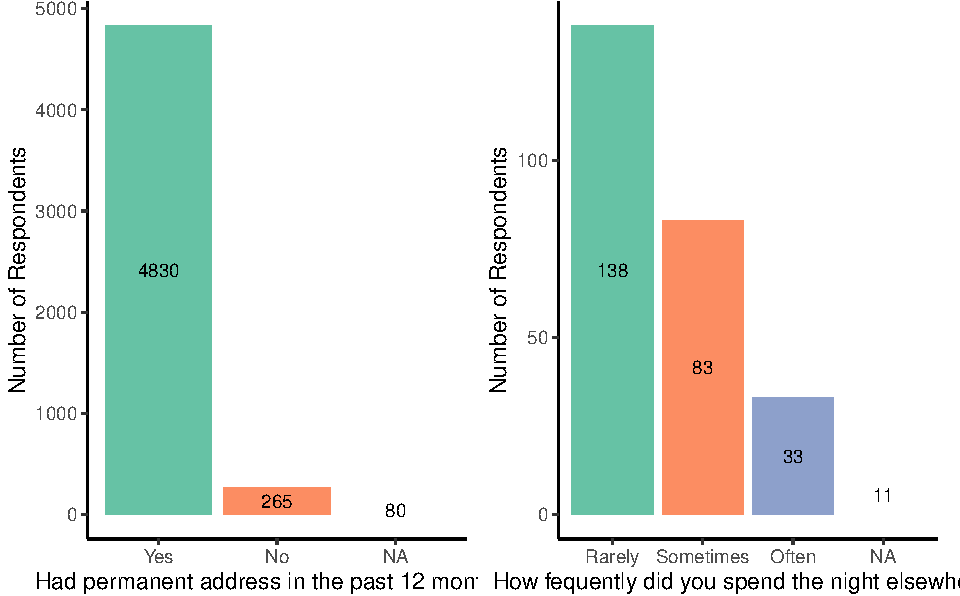
\includegraphics{final_phase2_report_files/figure-latex/unnamed-chunk-3-1} \end{center}

\hypertarget{distribution-of-food-insecurity-responses}{%
\subsubsection{Distribution of Food Insecurity Responses}\label{distribution-of-food-insecurity-responses}}

\begin{center}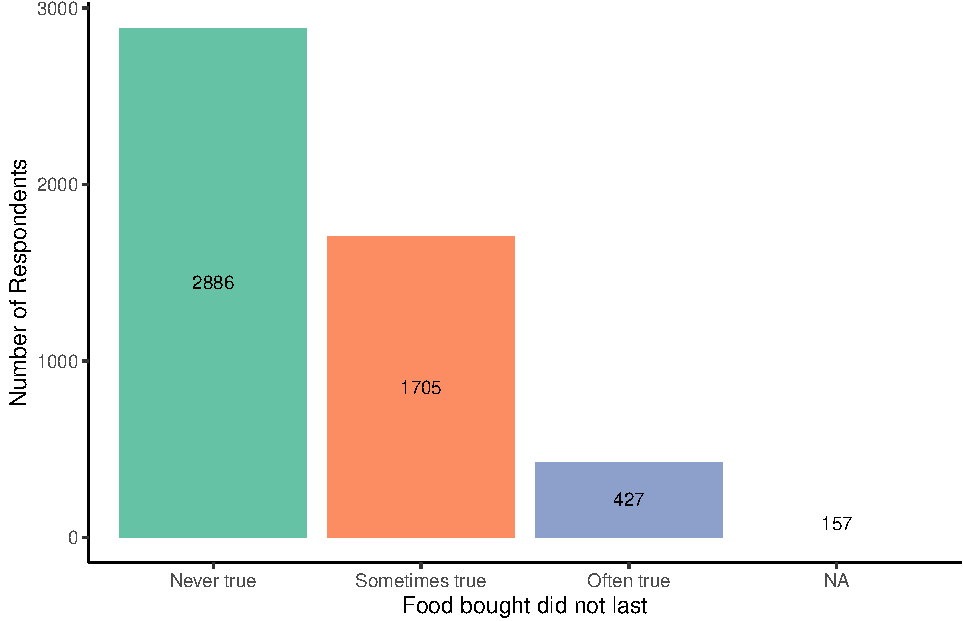
\includegraphics{final_phase2_report_files/figure-latex/unnamed-chunk-5-1} \end{center}

\begin{center}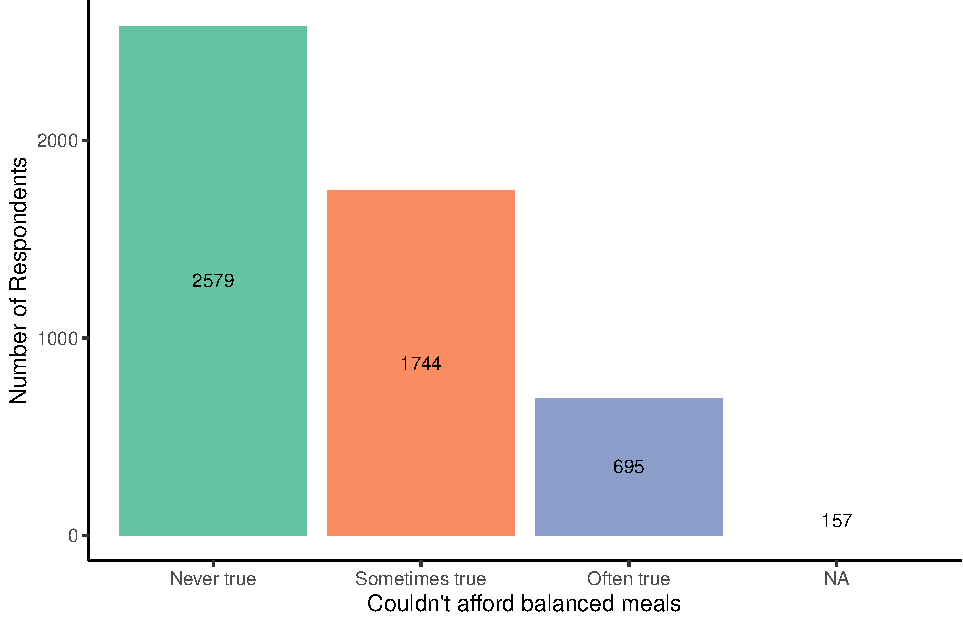
\includegraphics{final_phase2_report_files/figure-latex/unnamed-chunk-6-1} \end{center}

\begin{center}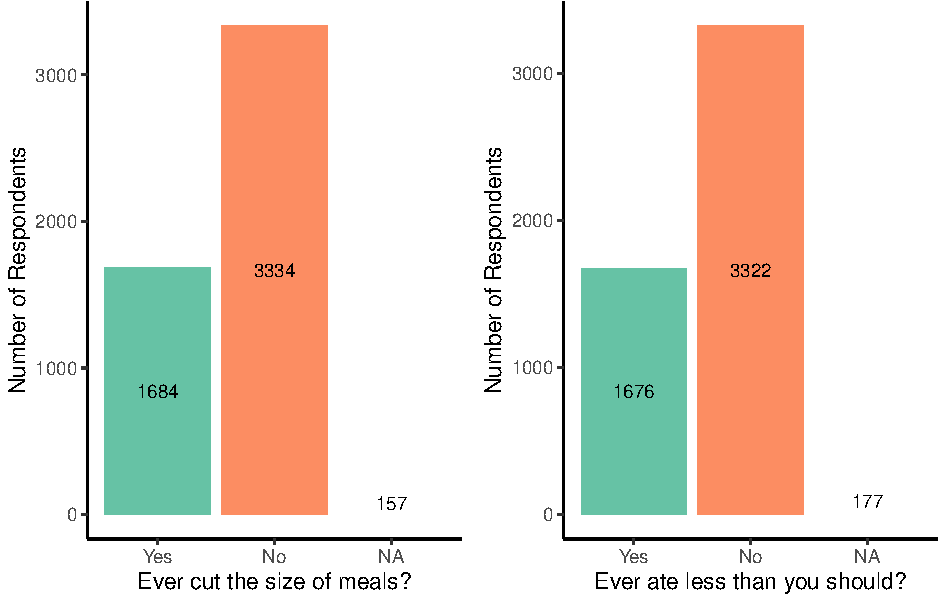
\includegraphics{final_phase2_report_files/figure-latex/unnamed-chunk-7-1} \end{center}

\begin{center}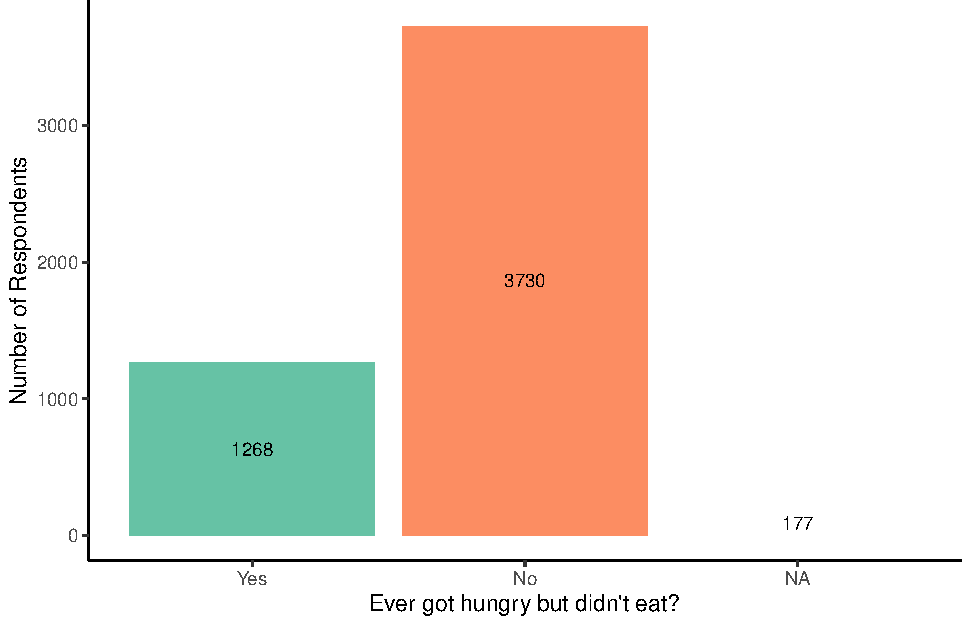
\includegraphics{final_phase2_report_files/figure-latex/unnamed-chunk-8-1} \end{center}

The table and graphs above display the number of missing values with missing percentages as well as the distribution of the potential response variables. From the results, the following observations were made:

\begin{itemize}
\item
  It is clear that all variables have some amount of missing observation given they are all above 50\%, hence a necessary missing data treatment is required.
\item
  The response variables also contains missing values, hence we filter all missing observation with respect to each response variable out and used the remaining data set for further imputation and analysis analysis.
\item
  The mice package aided in imputation the missing values in the predictor variables, specifically by using the median, mice was chosen because it is robust to data and its imputation style.
\item
  The selected response variables exhibited highly imbalanced classification. The imbalanced classification was treated with both sampling methods under the ROSE package.
\end{itemize}

\hypertarget{model-building}{%
\subsection{Model Building}\label{model-building}}

Given our data set and its structure, the following supervised classification machine learning algorithms were employed to obtained a predictive model for each given response variable;

\begin{itemize}
\item
  Logistic Regression
\item
  Linear Discriminant Analysis (LDA)
\item
  K-Nearest Neighbors (KNN)
\item
  Multivariate Adaptive Regression Splines (MARS)
\item
  Support Vector Machines with Linear Kernel (SVM Linear)
\item
  Support Vector Machines with Radial Basis Kernel (SVM Radial)
\end{itemize}

\hypertarget{partitioning-data-set}{%
\subsubsection{Partitioning data set}\label{partitioning-data-set}}

For the purpose of training and validation of each derived model ,and the estimation of the performance metrics, the entire data set was partitioned into training and testing in a ratio of 2/3 and 1/3 respectively.

\hypertarget{results-for-housing-insecurity-responses}{%
\subsubsection{Results for Housing Insecurity Responses}\label{results-for-housing-insecurity-responses}}

Here, we modeled housing insecurity as a response based on whether or not a respondent had a permanent address (permanent\_address) as well as whether or not a respondent spent the night elsewhere given that they did not have a permanent address in the past six months to the survey period (spent\_night\_elsewhere).

\textbf{Results for Permanent Address}

\begin{table}[H]

\caption{\label{tab:unnamed-chunk-9}Evaluation metrics for Permanent House Address  as a response variable}
\centering
\fontsize{12}{14}\selectfont
\begin{tabular}[t]{lcccccc}
\toprule
Model & Misclassification Rate & Accuracy & Sensitivity & Specificity & fbeta & AUC\\
\midrule
Logistic & 0.24 & 0.76 & 0.77 & 0.53 & 0.86 & 0.7058\\
LDA & 0.22 & 0.78 & 0.79 & 0.55 & 0.87 & 0.7149\\
KNN & 0.37 & 0.63 & 0.64 & 0.57 & 0.77 & 0.637\\
MARS & 0.2 & 0.8 & 0.82 & 0.48 & 0.89 & 0.7206\\
SVM Linear & 0.22 & 0.78 & 0.79 & 0.51 & 0.87 & 0.7151\\
SVM Radial & 0.17 & 0.83 & 0.85 & 0.45 & 0.91 & 0.7011\\
\bottomrule
\end{tabular}
\end{table}

Based on the table values our best initial models are SVM Radial and the MARS (earth) model from the permanent housing address response.\\

\begin{center}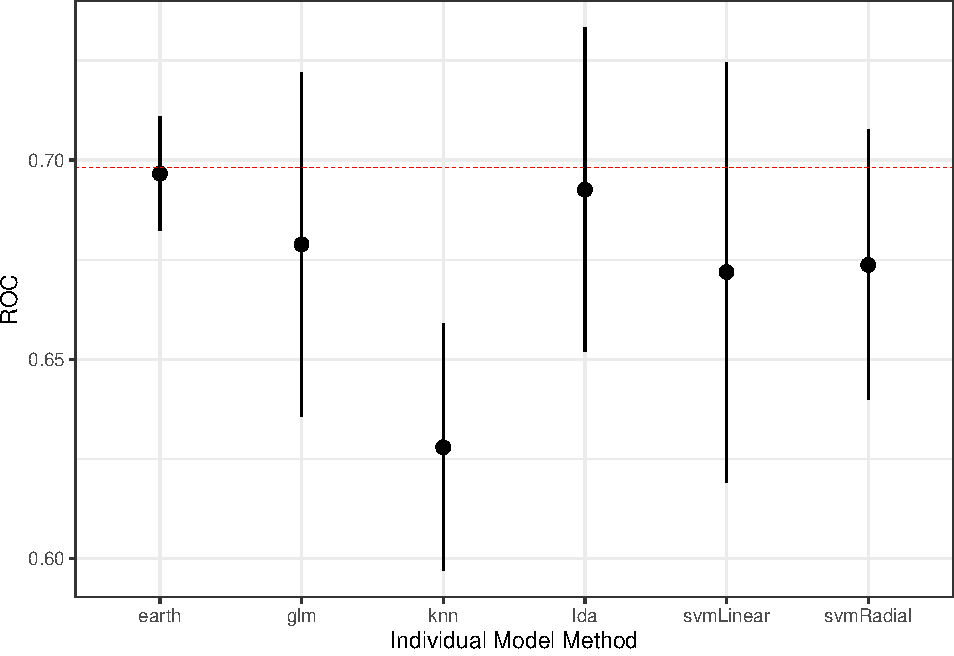
\includegraphics{final_phase2_report_files/figure-latex/unnamed-chunk-10-1} \end{center}

The ensemble model came up with the MARS (earth) model as the best performing model given its line of reference. Therefore, we confidently conclude that the MARS model which appeared at both our necessary and sufficient measure for selection criteria is the model predictive model for modeling the housing insecurity permanent address.\\

\begin{center}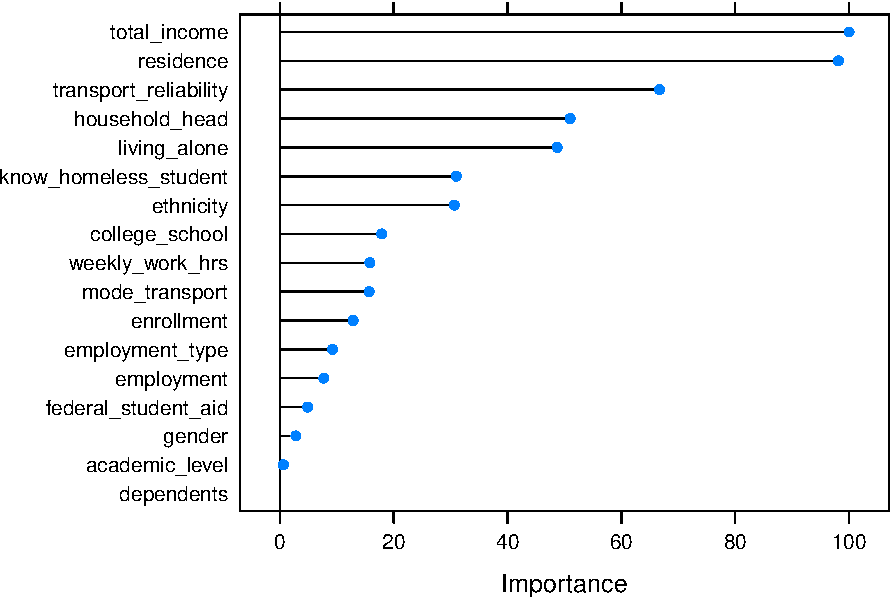
\includegraphics{final_phase2_report_files/figure-latex/unnamed-chunk-11-1} \end{center}

\begin{center}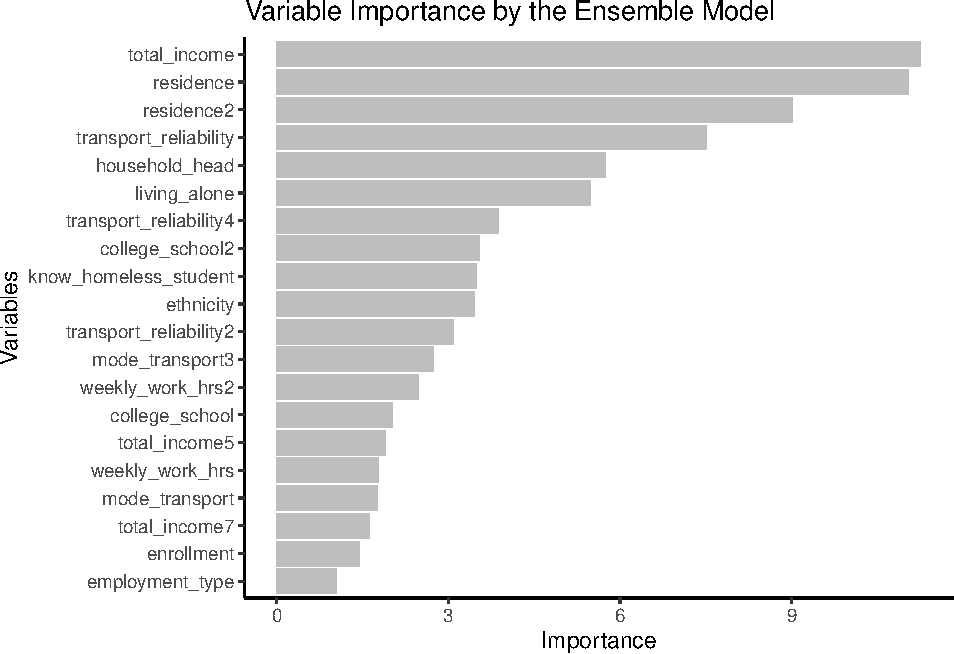
\includegraphics{final_phase2_report_files/figure-latex/unnamed-chunk-12-1} \end{center}

Our initial preferred model based on the evaluation metrics been SVM Radial would have total income, residence, transport reliability, household head, and living alone are the top five variables that accurately predicts the housing insecurity, with employment, federal aid, gender, and dependents been least of importance. However our final model by the ensemble method which is the MARS model also had same variables of most importance as that of the SVM radial. However this MARS model plot further classifies the important variable residence2 , transport reliability and college\_school2 as subgroups of importance.\\

\textbf{Results for Spending the night elsewhere}

\begin{table}[H]

\caption{\label{tab:unnamed-chunk-13}Evaluation metrics for Spent Night Elsewhere  as a response variable}
\centering
\fontsize{12}{14}\selectfont
\begin{tabular}[t]{lcccccc}
\toprule
Model & Misclassification Rate & Accuracy & Sensitivity & Specificity & fbeta & AUC\\
\midrule
Logistic & 0.54 & 0.46 & 0.35 & 0.56 & 0.37 & 0.5216\\
KNN & 0.45 & 0.55 & 0.49 & 0.6 & 0.49 & 0.5294\\
MARS & 0.45 & 0.55 & 0.65 & 0.47 & 0.56 & 0.5952\\
SVM Linear & 0.54 & 0.46 & 0.51 & 0.42 & 0.46 & 0.5012\\
SVM Radial & 0.51 & 0.49 & 0.54 & 0.44 & 0.49 & 0.5498\\
\bottomrule
\end{tabular}
\end{table}

Taking spending the night elsewhere, our initial best model is the MARS (earth) model given the table values, that is MARS model has the least misclassification, higher accuracy, higher fbeta, and higher AUC. However we add SVM radial to our best model since its comes next to the MARS model for example that AUC and fbeta.\\

\begin{center}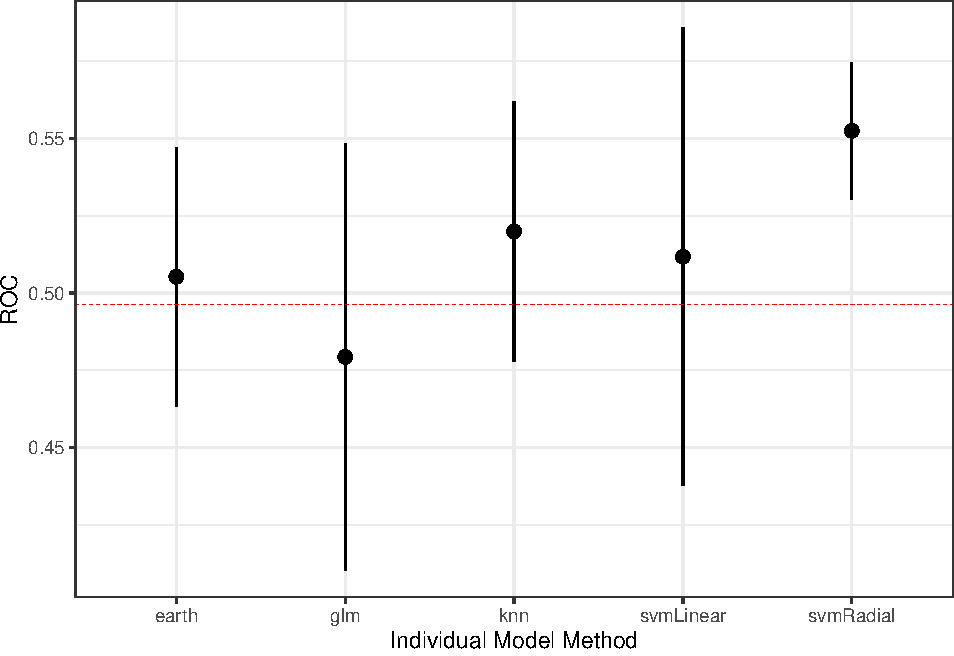
\includegraphics{final_phase2_report_files/figure-latex/unnamed-chunk-14-1} \end{center}

According to the ensemble modeling, the SVM Radial is the best given the reference line. Hence the SVM Radial becomes our best model given spending the night elsewhere as the response variable.\\

\begin{center}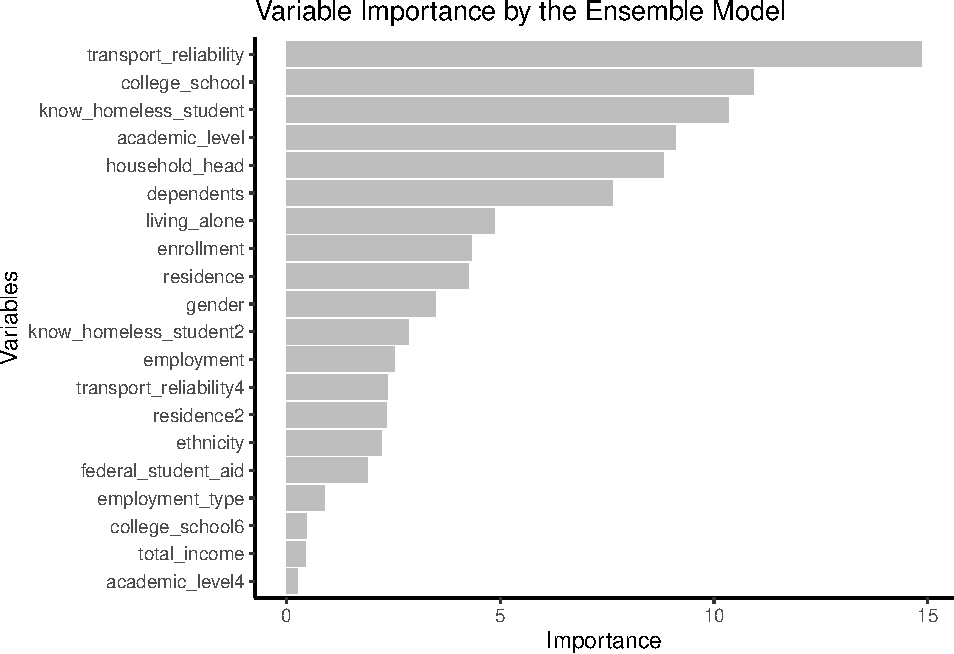
\includegraphics{final_phase2_report_files/figure-latex/unnamed-chunk-15-1} \end{center}

\begin{center}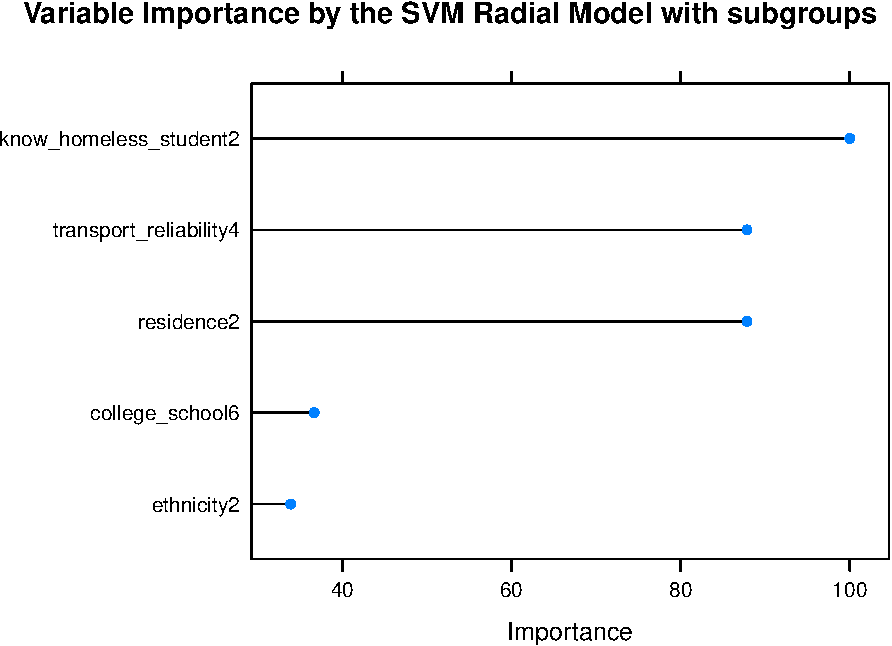
\includegraphics{final_phase2_report_files/figure-latex/unnamed-chunk-16-1} \end{center}

According to our variable of an important plot from the best model (SVM radial), the top 5 variables that determine housing insecurity are transport reliability, college, known homeless students, academic level, and household head. Also know homeless student2, residence2, transport reliability 4, college school6 and ethnicity2 are the subgroups of importance.\\

\hypertarget{results-for-food-insecurity-responses}{%
\subsubsection{Results for Food Insecurity Responses}\label{results-for-food-insecurity-responses}}

In this section, we report results for modeling food insecurity in terms response variables based on survey questions as described below:

\begin{itemize}
\item
  \textbf{Food Insecurity I}: ``The food that I bought just didn't last, and I didn't have money to get more.'' Was that often, sometimes, or never true for you in the last 12 months? (FI\_q26).
\item
  \textbf{Food Insecurity II}: ``I couldn't afford to eat balanced meals.'' Was that often, sometimes, or never true for you in the last 12 months? (FI\_q27).
\item
  \textbf{Food Insecurity III}: In the last 12 months, since (today's date), did you ever cut the size of your meals or skip meals because there was not enough money for food? (FI\_q28).
\end{itemize}

\begin{itemize}
\tightlist
\item
  \textbf{Food Insecurity IV}: In the past 12 months, were you ever hungry but didn't eat because there wasn't enough money for food? (FI\_q31).
\end{itemize}

Though Food Insecurity I and II originally had three levels (Often true, Sometimes true, and Never true), we modeled them as dichotomous responses where the ``Often true'' and ``Sometimes true'' levels were put in a ``Yes'' group as a sign of food insecurity, while the ``Never true'' level was classified as a ``No'' group for respondents not at the risk of food insecurity.

\textbf{Results for Food Insecurity Response I}

\begin{table}[H]

\caption{\label{tab:unnamed-chunk-17}Evaluation metrics for Food Insecurity I  as a response variable}
\centering
\fontsize{12}{14}\selectfont
\begin{tabular}[t]{lcccccc}
\toprule
Model & Misclassification Rate & Accuracy & Sensitivity & Specificity & fbeta & AUC\\
\midrule
Logistic & 0.33 & 0.67 & 0.66 & 0.67 & 0.64 & 0.7342\\
LDA & 0.34 & 0.66 & 0.65 & 0.67 & 0.63 & 0.7335\\
KNN & 0.36 & 0.64 & 0.58 & 0.68 & 0.59 & 0.6747\\
MARS & 0.34 & 0.66 & 0.66 & 0.66 & 0.64 & 0.7319\\
SVM Linear & 0.34 & 0.66 & 0.66 & 0.66 & 0.63 & 0.7314\\
SVM Radial & 0.33 & 0.67 & 0.66 & 0.67 & 0.64 & 0.7322\\
\bottomrule
\end{tabular}
\end{table}

Based on the table values and the evaluation metric criteria, with the exception of knn model , all the others are preferred as our initial best models.\\

\begin{center}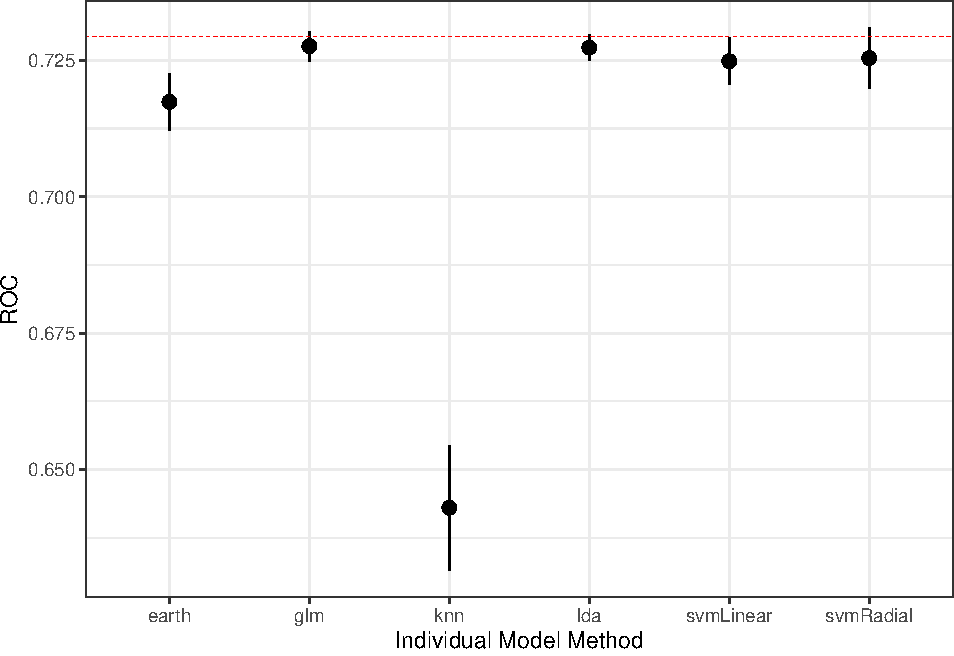
\includegraphics{final_phase2_report_files/figure-latex/unnamed-chunk-18-1} \end{center}

From the ensemble model, both glm and LDA are considered the best model for predicting food insecurity response 1, however, we decide on logistics regression as our best model.\\

\begin{center}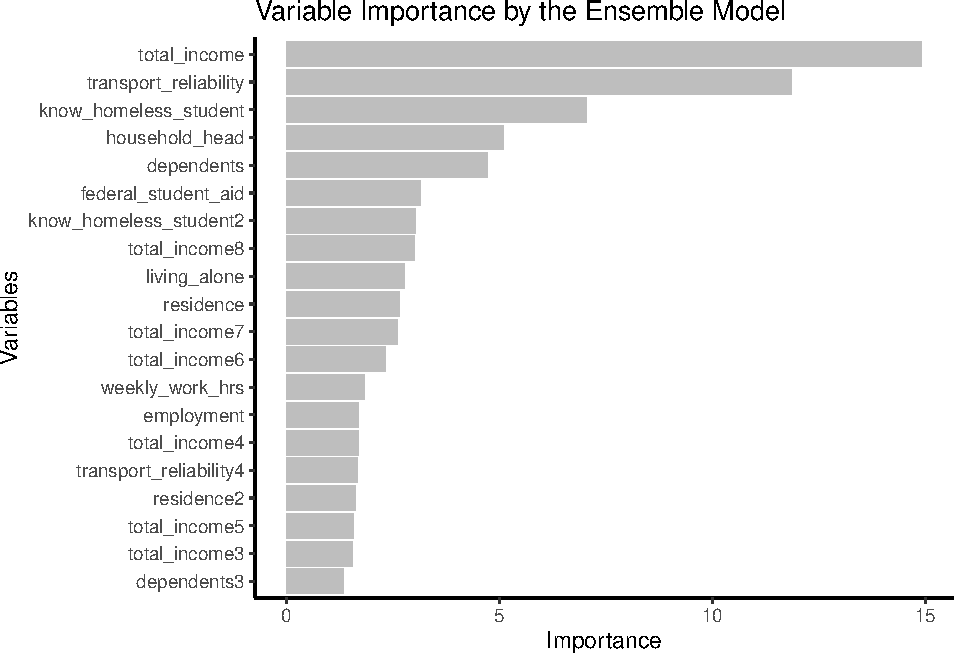
\includegraphics{final_phase2_report_files/figure-latex/unnamed-chunk-19-1} \end{center}

Using glm as our best model the variable of importance or factor that predict food insecurity 1 as response are total income, transport reliability, know homeless student, household head and dependents.\\

\begin{center}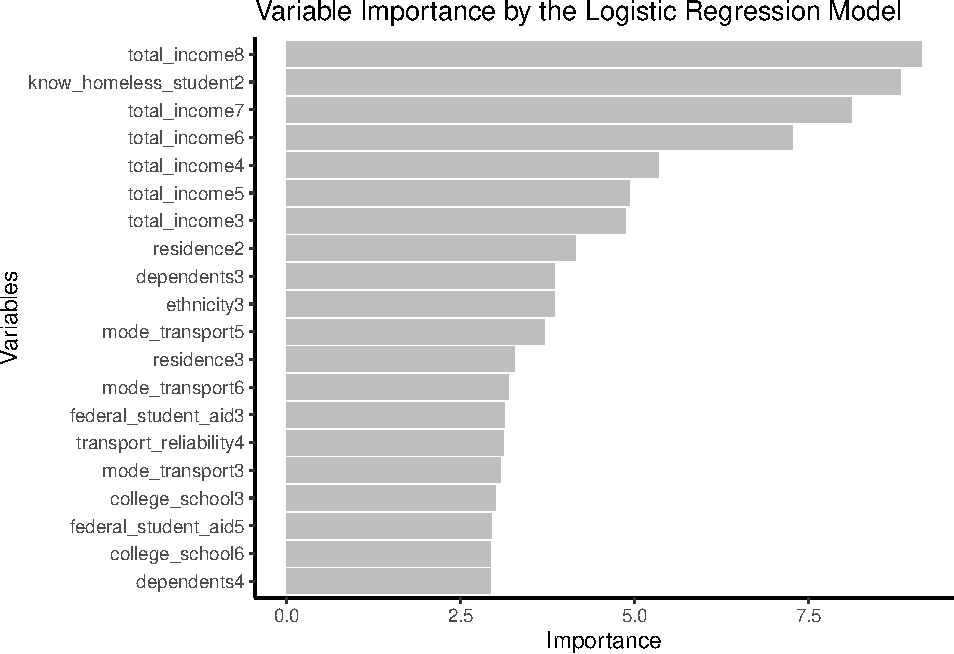
\includegraphics{final_phase2_report_files/figure-latex/unnamed-chunk-20-1} \end{center}

Given the plot above, the top 5 subgroups are total income8, know homeless student 2, total income 7, residence2, and ethnicity3.\\

\textbf{Results for Food Insecurity Response II}

\begin{table}[H]

\caption{\label{tab:unnamed-chunk-21}Evaluation metrics for Food Insecurity II  as a response variable}
\centering
\fontsize{12}{14}\selectfont
\begin{tabular}[t]{lcccccc}
\toprule
Model & Misclassification Rate & Accuracy & Sensitivity & Specificity & fbeta & AUC\\
\midrule
Logistic & 0.34 & 0.66 & 0.64 & 0.67 & 0.66 & 0.7123\\
LDA & 0.34 & 0.66 & 0.65 & 0.67 & 0.66 & 0.7132\\
KNN & 0.37 & 0.63 & 0.56 & 0.7 & 0.6 & 0.6689\\
MARS & 0.35 & 0.65 & 0.64 & 0.65 & 0.65 & 0.7078\\
SVM Linear & 0.35 & 0.65 & 0.64 & 0.67 & 0.65 & 0.7116\\
SVM Radial & 0.35 & 0.65 & 0.63 & 0.67 & 0.65 & 0.7113\\
\bottomrule
\end{tabular}
\end{table}

Modeling food insecurity 2 as response, the best initial models are all models apart from the knn model.\\

\begin{center}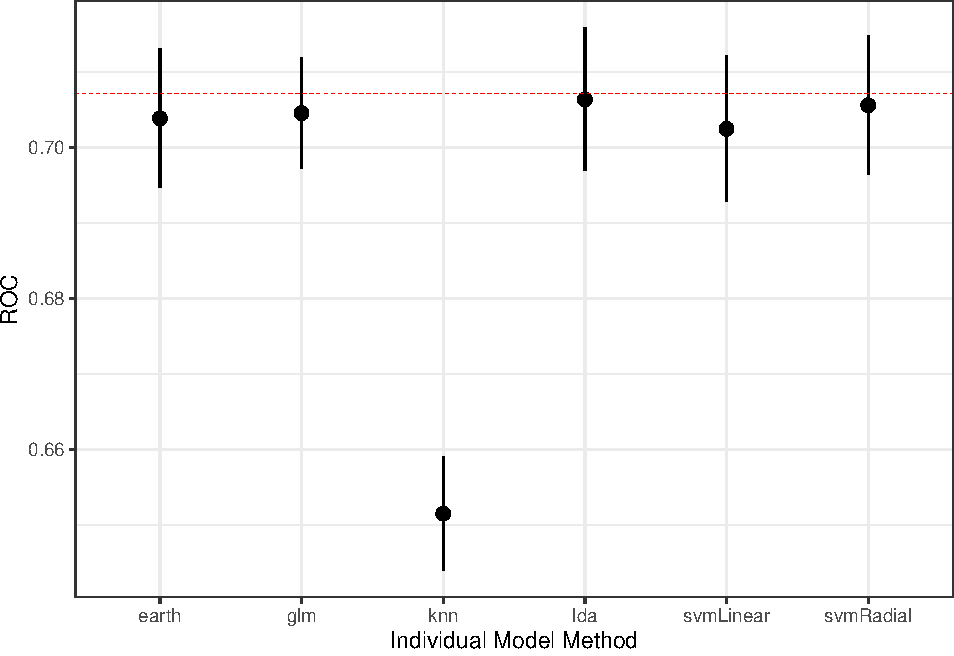
\includegraphics{final_phase2_report_files/figure-latex/unnamed-chunk-22-1} \end{center}

The best model from the ensemble model is the LDA, however, the SVM Radial can as well the best model given that it is closer to the line of reference as indicated from the plot above.\\

\begin{center}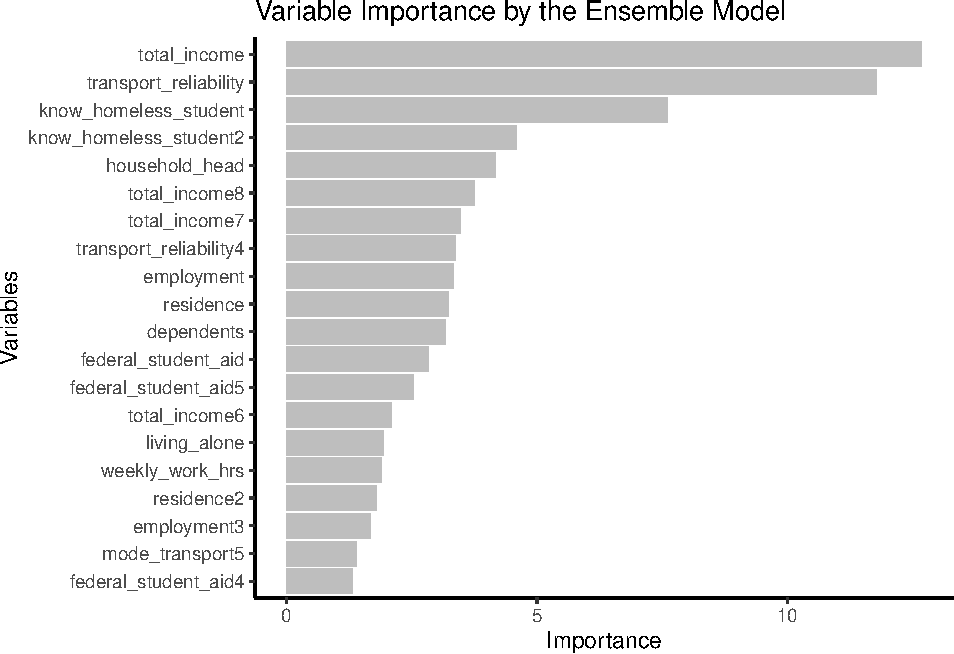
\includegraphics{final_phase2_report_files/figure-latex/unnamed-chunk-23-1} \end{center}

The plot above indicates that treating food insecurity 2 as a response through the LDA model by ensemble model, the 5 most important factors are total income, transport reliability, know homeless student, household head, and employment.\\

\begin{center}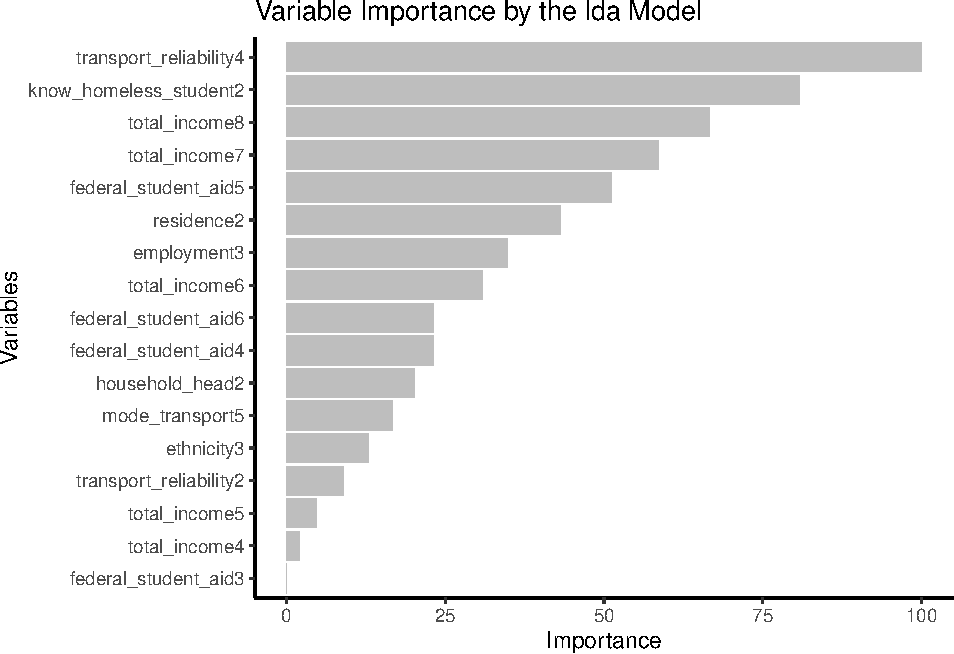
\includegraphics{final_phase2_report_files/figure-latex/unnamed-chunk-24-1} \end{center}

Given the plot above, the top 5 subgroups are transport reliability4, know homeless student2, total income8, federal student aid5, and residence2.\\

\textbf{Results for Food Insecurity Response III}

\begin{table}[H]

\caption{\label{tab:unnamed-chunk-25}Evaluation metrics for Food Insecurity III  as a response variable}
\centering
\fontsize{12}{14}\selectfont
\begin{tabular}[t]{lcccccc}
\toprule
Model & Misclassification Rate & Accuracy & Sensitivity & Specificity & fbeta & AUC\\
\midrule
Logistic & 0.35 & 0.65 & 0.59 & 0.68 & 0.55 & 0.7004\\
LDA & 0.34 & 0.66 & 0.62 & 0.69 & 0.57 & 0.7017\\
KNN & 0.38 & 0.62 & 0.54 & 0.67 & 0.51 & 0.6515\\
MARS & 0.35 & 0.65 & 0.59 & 0.68 & 0.55 & 0.6975\\
SVM Linear & 0.34 & 0.66 & 0.6 & 0.69 & 0.56 & 0.7006\\
SVM Radial & 0.33 & 0.67 & 0.59 & 0.71 & 0.56 & 0.7033\\
\bottomrule
\end{tabular}
\end{table}

Given the table values of evaluation metric criteria, our initial best models are all but knn and MARS.\\

\begin{center}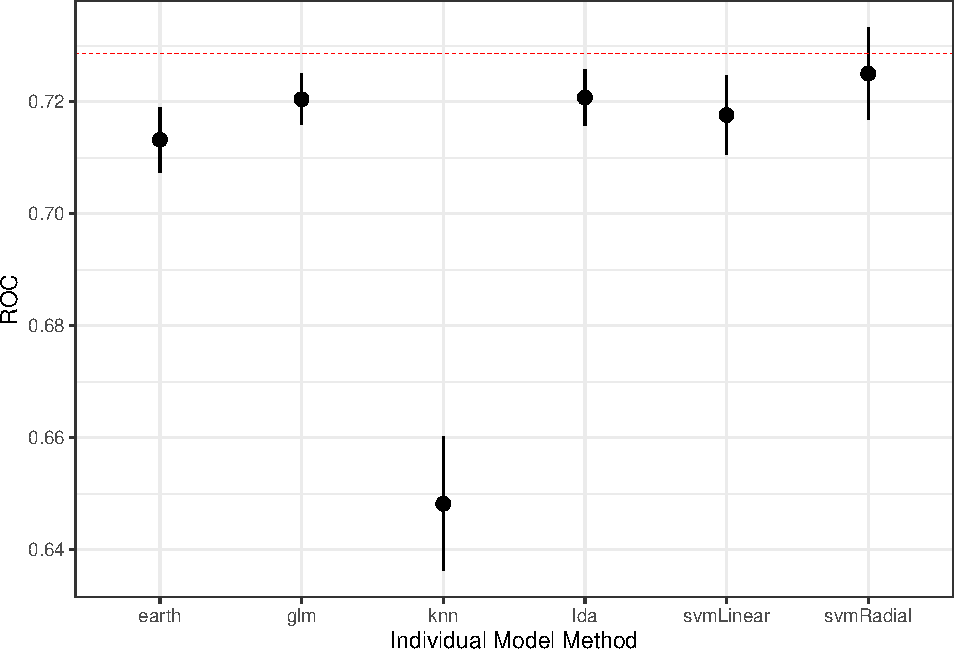
\includegraphics{final_phase2_report_files/figure-latex/unnamed-chunk-26-1} \end{center}

The final best model through the ensemble method is the SVM Radial for the food insecurity 3.\\

\begin{center}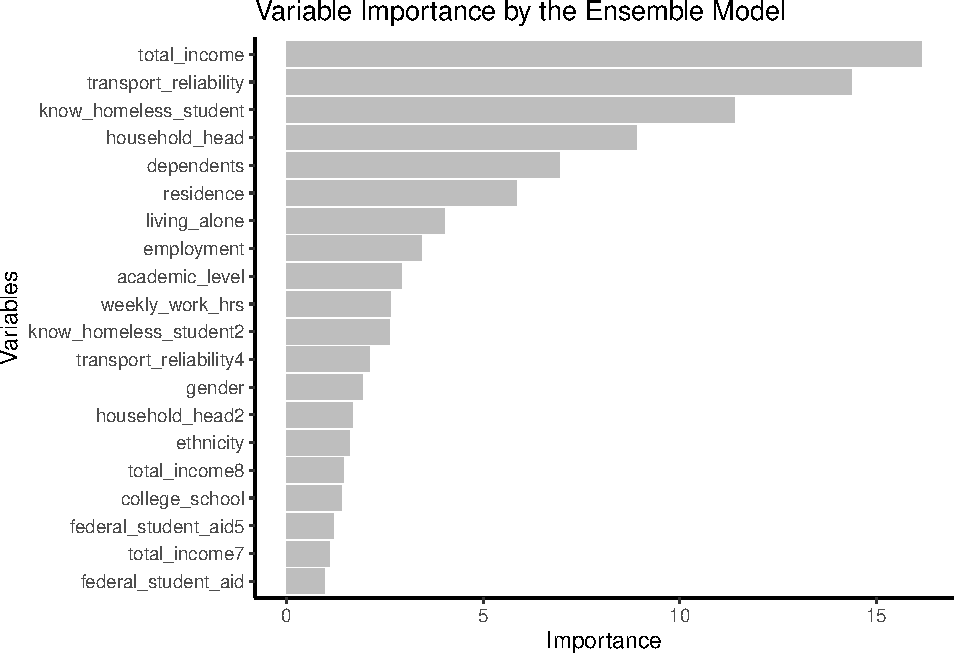
\includegraphics{final_phase2_report_files/figure-latex/unnamed-chunk-27-1} \end{center}

The plot above indicates that treating food insecurity 3 as a response through the SVM Radial model by ensemble model, the 5 most important factors are total income, transport reliability, know homeless student, household head, and depedents.\\

\begin{center}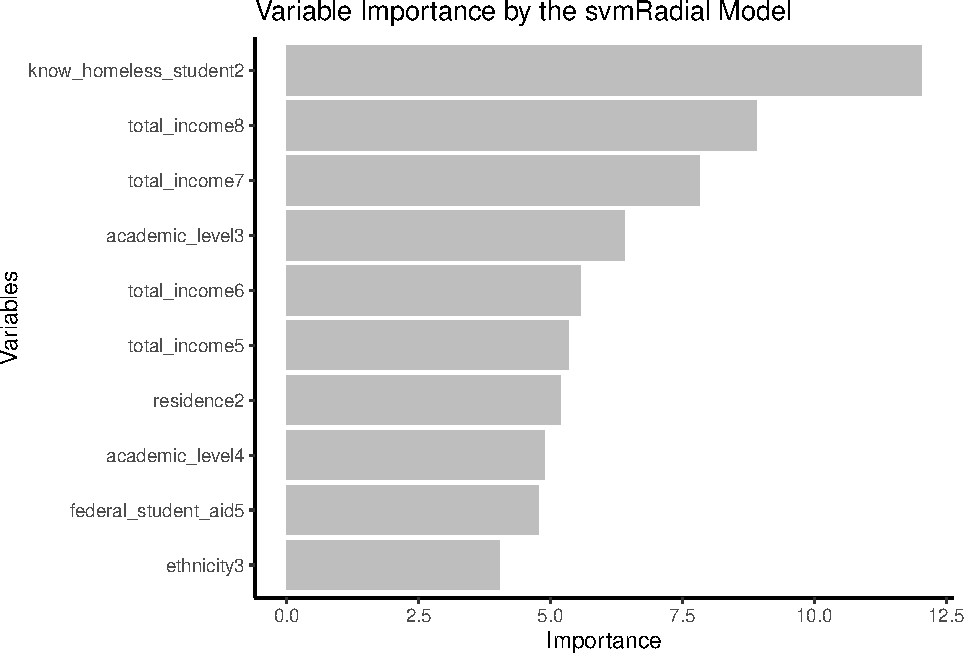
\includegraphics{final_phase2_report_files/figure-latex/unnamed-chunk-28-1} \end{center}

Given the plot above for food insecurity 3, the top 5 subgroups are know homeless student2, total income8, total income7, academic level3, and residence2.

\textbf{Results for Food Insecurity Response IV}

\begin{table}[H]

\caption{\label{tab:unnamed-chunk-29}Evaluation metrics for Food Insecurity V  as a response variable}
\centering
\fontsize{12}{14}\selectfont
\begin{tabular}[t]{lcccccc}
\toprule
Model & Misclassification Rate & Accuracy & Sensitivity & Specificity & fbeta & AUC\\
\midrule
Logistic & 0.31 & 0.69 & 0.65 & 0.7 & 0.52 & 0.7325\\
LDA & 0.32 & 0.68 & 0.65 & 0.69 & 0.51 & 0.7312\\
KNN & 0.38 & 0.62 & 0.55 & 0.65 & 0.43 & 0.6433\\
MARS & 0.32 & 0.68 & 0.63 & 0.69 & 0.5 & 0.7262\\
SVM Linear & 0.32 & 0.68 & 0.65 & 0.7 & 0.51 & 0.731\\
SVM Radial & 0.3 & 0.7 & 0.62 & 0.73 & 0.52 & 0.7375\\
\bottomrule
\end{tabular}
\end{table}

Our best models according the evaluation metrics criteria are glm and SVM Radial for food insecurity response 4.\\

\begin{center}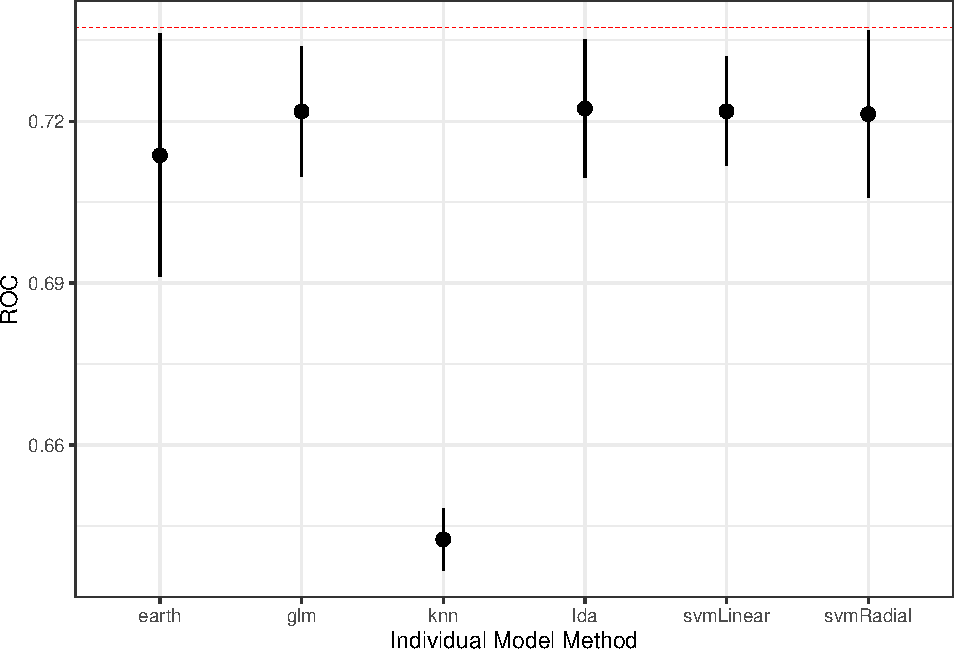
\includegraphics{final_phase2_report_files/figure-latex/unnamed-chunk-30-1} \end{center}

Now according to the ensemble method, both initial best models are best for predicting the response variable, however, we decided on the glm model as per the ensemble model.\\

\begin{center}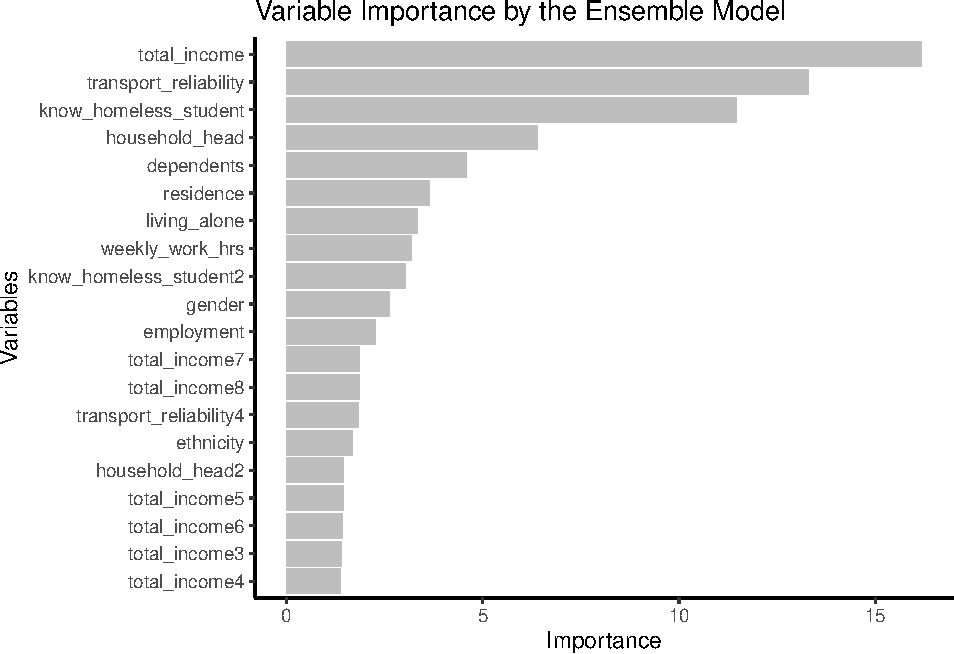
\includegraphics{final_phase2_report_files/figure-latex/unnamed-chunk-31-1} \end{center}

The plot above indicates that treating food insecurity 4 as a response through the glm model by ensemble model, the 5 most important factors are total income, transport reliability, know homeless student, household head, and dependents.\\

\begin{center}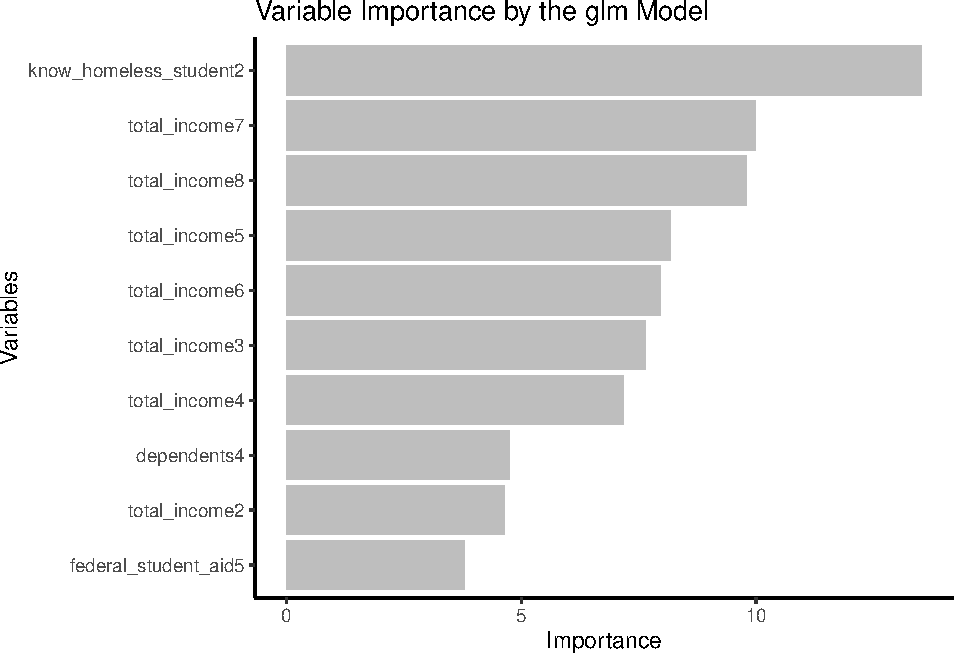
\includegraphics{final_phase2_report_files/figure-latex/unnamed-chunk-32-1} \end{center}

Given the plot above for food insecurity 3, the top 10 subgroups involves known homeless student2, total income (2,3 - 8), dependents4 and federal student aid5.

\section{Methodology}

This section serves to provide a road map to the approaches our group adopted and executed in terms of our analysis.

\subsection{Exploratory Data Analysis}

In this section, we provided descriptive analyses of the data including numerical summaries and graphical displays as a first-hand insight into the data to help ourselves and our audiences to better understand the underlying dataset. We primarily looked at the distributions of our target variables and all the predictor variables.

In terms of the types of graphs or visualizations, we considered segmented or comparative bar graphs. We critically assessed these graphs and settled on a few which help us to effectively tell a compelling story about the data.

\begin{itemize}
\item
  \textbf{Cross Tabulations (Contingency Tables)}: Provide numerical summary of how responses differ by some categories.
\item
  \textbf{Bar graphs (Segmented/Comparative bar graphs)}: To explore how the available categorical predictors are distributed across the levels of the target or response variable.
\end{itemize}

\hypertarget{missing-dataoutliers-and-their-treatments}{%
\subsubsection{Missing Data/Outliers and their treatments}\label{missing-dataoutliers-and-their-treatments}}

The available data was inspected for missing and unusual values. The missing data and/or outlying data identified from our data preprocessing and exploratory analysis was treated appropriately depending on the nature of the missingness and the information we were able to gather about the possible reasons for the missingness or unusual values. In such instnaces, the \texttt{mice} package was used for data imputation.

\hypertarget{modeling-approaches}{%
\subsection{Modeling Approaches}\label{modeling-approaches}}

\hypertarget{data-partitioning}{%
\subsubsection{Data Partitioning}\label{data-partitioning}}

For the purpose of predictions or testing on the machine learning algorithm models or estimation of the evaluation metrics for the best model selection, the entire dataset were partitioned into training data and testing data. The training data would be used to fit the models and the testing data was used to derive the metrics for model selection or testing.

\subsubsection{Predictive Models}

In this part of the analysis, since the nature of the task present a classification problem, we fit several classification models to the target variable as a function of all the possible predictors we selected from the original dataset. All the models considered are \emph{supervised} learning algorithms. Candidate models included Logistic regression, Linear Discriminant Analysis (LDA), K-nearest neighbors (KNN), Support Vector Machines/Classifiers, Multivariate Adaptive Regression Splines.

\hypertarget{logistic-regression}{%
\paragraph{\texorpdfstring{Logistic Regression }{Logistic Regression  }}\label{logistic-regression}}

Logistic Regression is very simple and one of the mostly used traditional machine learning algorithms. It is a statistical model for predicting binary classes. However, as remarked by James, Witten, Hastie, and Tibshirani (\protect\hyperlink{ref-james2013introduction}{2013}), multiple-class extension of Logistic Regression exists but \emph{Discriminant Analysis} models are commonly used in place of it. The dependent variable in here follows Bernoulli distribution. Logistic Regression model uses the logistic function or sigmoid function for predictive modeling of the given problem, which takes value between 0 and 1. 1 will be predicted if the curve goes to positive infinity and 0 if it goes to negative infinity. The logistic Regression model performs the predictive analysis based on the relationship between the binary dependent variable and the other one or more independent variables from the given dataset.

\hypertarget{k-nearest-neighbors-classifier}{%
\paragraph{K-Nearest Neighbors Classifier}\label{k-nearest-neighbors-classifier}}

K-nearest neighbors regression (KNN regression) is one of the simplest and best-known
non-parametric methods. Unlike the Logistic Regression, no assumptions are made about the shape of the decision boundary. Therefore, we can expect this approach to dominate Logistic Regression when the decision boundary is highly non-linear. It uses a distance metric such as the Euclidean distance for separation between points in the feature space. In the KNN classification model, the prediction is purely based on neighbor data values without any assumption on the dataset. The \(K\) in the name of the model represents the number of nearest neighbor data values. This parameter can be tuned to find an optimal value. Based on \(K\), the decision is made by the KNN algorithm on classifying the given dataset.

\hypertarget{support-vector-machines-svm}{%
\paragraph{\texorpdfstring{Support Vector Machines (SVM) }{Support Vector Machines (SVM)  }}\label{support-vector-machines-svm}}

Support Vector Machines; SVM is a great classification machine learning model for classifying data of clear classes. Also does not require a predetermined cutoff point for prediction. Given a set of training examples, each marked as belonging to one of two categories, an SVM training algorithm builds a model that assigns new examples to one category or the other, making it a non-probabilistic binary linear classifier (although methods such as Platt scaling exist to use SVM in a probabilistic classification setting). SVM maps training examples to points in space so as to maximize the width of the gap between the two categories. New examples are then mapped into that same space and predicted to belong to a category based on which side of the gap they fall (Wikipedia, \protect\hyperlink{ref-wikipedia}{2021}).
We will consider using this classification model because it is versatile and effective in high dimensional spaces. They are versatile in the sense that different Kernel functions can be specified for the decision function. Common kernels include polynomial kernels and radial kernels. Support vector classifiers are also able to address the problem of possibly non-linear boundaries between classes. We will try at least three kernel SVM for this analysis noticeably, the Linear SVM and two Non-Linear kernels SVM such as the Gaussian radial basis function (RBF) and Polynomial kernel SVM through packages such as caret and kernlab.

\hypertarget{multivariate-adaptive-regression-splines}{%
\paragraph{Multivariate Adaptive Regression Splines}\label{multivariate-adaptive-regression-splines}}

We employed one MARS model with an appropriate set-up of parameters as another baseline classifier. The MARS algorithm is also suitable for a large number of predictor variables, robust to outliers, it automatically detects interactions between variables, and despite its complexity, it is an efficient fast algorithm. However, it is susceptible to overfitting, more difficult to understand and interpret as against others, and not good with missing data.

\hypertarget{model-validation}{%
\subsection{Model Validation}\label{model-validation}}

The k-fold cross-validation resampling technique was used to validate our prediction models.

\hypertarget{performanceevaluation-metrics}{%
\subsection{Performance/Evaluation Metrics}\label{performanceevaluation-metrics}}

The following metrics were employed to examine the performance of the models for best predictive power.

\hypertarget{f-beta-score-f_beta}{%
\subsubsection{\texorpdfstring{F-beta Score (\(F_\beta\))}{F-beta Score (F\_\textbackslash beta)}}\label{f-beta-score-f_beta}}

The F-beta score or F-beta measure is the weighted harmonic mean of precision and recall, reaching its optimal value at 1 and its worst value at 0. It turns the F-measure into a configurable single-score metric for evaluating a binary classification model based on the predictions made for the positive class. The beta parameter determines the weight of recall and precision in the combined score. \(\beta < 1\) lends more weight to precision, while \(\beta > 1\) favors recall. That is, a smaller beta value, such as 0.5, gives more weight to precision and less to recall, whereas a larger beta value, such as 2.0, gives less weight to precision and more weight to recall in the calculation of the score. It is a useful metric to use when both precision and recall are important but slightly more attention is needed on one or the other, such as when false negatives are more important than false positives, or the reverse (Machine Learning Mastery (\protect\hyperlink{ref-MLM}{2021}), Scikit Learn (\protect\hyperlink{ref-scikit_learn}{2021})).

We can compute the F-beta score by

\[
  F_\beta = \frac{(1 + \beta^2) * Precision * Recall}{\beta^2 * Precision + Recall},
\]
where \textbf{precision} and \textbf{recall} are defined below.

The choice of the beta parameter will be used in the name of the F-beta score. For example, a \(\beta\) value of 1 is referred to as the \(F_1\)-measure or the \(F_1\) score. A \(\beta\) value of 2 is referred to as \(F_2\)-measure or \(F_2\)-score.

\textbf{Precision}

Precision is a metric that quantifies the number of correct positive predictions made. It is computed as the ratio of correctly predicted positive classes divided by the total number of positive classes that were predicted as in the formula below.

\[
\text{Precision} = \frac{TP}{TP + FP} = \frac{\text{True Positives}}{\text{Total Predicted Positives}}
\]

\textbf{Recall}

Recall is a metric that quantifies the number of correct positive predictions made out of all positive predictions that could have been made. The intuition for recall is that it is not concerned with false positives and it minimizes false negatives (Machine Learning Mastery, \protect\hyperlink{ref-MLM}{2021}). It is calculated as

\[
\text{Recall} = \frac{\text{True Positives}}{\text{True Positives} + \text{True Negatives}} = \frac{TP}{TP + NP}
\]

\hypertarget{area-under-the-receiver-operator-curve-auroc}{%
\subsubsection{Area Under the Receiver Operator Curve (AUROC)}\label{area-under-the-receiver-operator-curve-auroc}}

The AUROC curve is a graphical illustration of the performance of the prediction model. The
ROC curve is the relationship between the recall and precision over varying threshold values. The threshold is the positive predictions of the model. The AUROC curve is plotted by keeping the x-axis a false positive rate and the y-axis as a true positive rate. Its value ranges from 0 to 1 (Theerthagiri, Jeena Jacob, Usha Ruby, and Yendapalli, \protect\hyperlink{ref-theerthagiri2021prediction}{2021}).

\hypertarget{model-selection}{%
\subsubsection{Model Selection}\label{model-selection}}

Base on the metrics calculated using the trained models and testing data for each classifier algorithm, the best model was selected, for instance, the model with the highest AUROC be best among the others, however, AUROC alone is not the measure for selection, hence a table other performance measures together with the AUC were used to estimate the one with the best performance across all metrics.

\hypertarget{model-deployment}{%
\subsection{Model Deployment}\label{model-deployment}}

To aid easy deployment and implementation of our proposed model(s), we planned to develop a web application with the R Shiny App package.This dashboard was to serve as an effective form of communicating our results to our client and other audiences. This was to provide among other features the flexibility to interact with the visualizations and models to assess performance based on changing parameters. We were aiming at an application similar to the online prediction tool developed by Dominguez-Rodriguez et al. (\protect\hyperlink{ref-dominguez2021bayesian}{2021}). Unfortunately, due to time constraint we were unable to develop such a communication tool.

\section{Background}

In this section, we provide an overview of Food and Housing Insecurity in Colleges in the U.S. in addition to the challenges faced by households in America. Also, we provide a description of the surveyed data obtained by The University of Texas at El Paso, processing of data cleaning and variable description.

This section primarily provides a background to the study by means of an overview of food insecurity and housing insecurity in the US in general and at El Paso, the satellite region of our target population, in particular.

\hypertarget{overview-of-the-study}{%
\subsection{Overview of the study}\label{overview-of-the-study}}

This project is aimed at analyzing data based on a survey constructed in summer 2019 and 2020 by a team of researchers at UTEP (Moya, Crouse, Schober, Wagler) to assess the state of food and housing insecurity among UTEP students. A slightly modified version of the survey was administered summer 2020. In this work, we seek to assess whether there are any changes to food and housing insecurities since 2019. This is particularly important since the worldwide pandemic hit during this period. The primary and secondary research questions are listed below.

\begin{enumerate}
\def\labelenumi{\arabic{enumi}.}
\item
  \textbf{Primary Research Question}: What factors are associated with food insecurity (FI) and housing insecurity (HI) among UTEP students?
\item
  \textbf{Secondary Research Question}: Which subpopulations of students are most at risk for FI and HI at UTEP?
\end{enumerate}

There are two phases to the project, phase I is concerned with the primary research question while phase II will be based on the secondary research question.

\hypertarget{overview-of-food-insecurity}{%
\subsection{Overview of Food Insecurity}\label{overview-of-food-insecurity}}

Food insecurity is defined by the United States Department of Agriculture (USDA) as the lack of consistent access to enough food for active healthy life. It can also be defined as a physical discomfort, thus the definition can relate to an individual or a family's lack of resources to obtain enough food for a healthy living. With the increasing spread of COVID-19, and many Americans losing their jobs, one of America's challenge worsened: hunger.During this period, communities and colleges in America in particular faced the longest queue's for food compared to past years.

According to the USDA, 13.7 million or 10.5\% of all households in the U.s. experienced food insecurity at some point during the COVID-19 pandemic. In addition, it was observed that, nearly 40\% of college students were food insecure. That means,24 of every 60 students are food insecure. After several years of research on food insecurity, researchers discovered food insecurity as a likelihood to deter college students from completing their degree.

Further research from USDAS stated over the past 20 years and a study completed in 2017 showed that, racial minorities, first-generation students, low income students, student with children and LGBTQ+ students are highly affected by COVID-19. These variables were included in analyzing the factors affecting food insecurities at UTEP.

\hypertarget{overview-of-housing-insecurity}{%
\subsection{Overview of Housing Insecurity}\label{overview-of-housing-insecurity}}

Housing insecurities includes difficulty in paying for living expense, overcrowding, substandard living and frequently moving out. Though housing insecurities can affect anyone, lower income families are known to be highly impacted since they pay high proportion of their lower income on high cost rent.

According to a 2019 report by The Hope Center for college, Communities and Justice, nearly 3 out of 5 students experience having insecurities in 2018. Also, 14\% of 4 year student reported experiencing homelessness. Despite the many challenges of housing insecurities, the impact of COVID-19 have increased the likelihood of homelessness among college students. For example, many students lost their jobs and financial due to COVID-19 pandemic.

\subsection{Data Description}

\subsubsection{Data cleaning and naming of variables}

In this section, we provide a brief description of the data for prediction and a method for renaming and collapsing the variables. The initial data from the survey comprises 12,536 observations with 104 columns. From the data, we observed enrollment and employment as the variables with the minimum number of missing values. In preparation of our data for modeling, we excluded the following questions from the our analysis: respondent ID, the age of the respondent, what pronouns do you use to describe yourself, where do you live, and variables associated with changes due to COVID-19. Table 1 shows the recoded names of the variables we considered in our analysis and their corresponding descriptions based on the survey questions.

\begin{table}[H]

\caption{\label{tab:variables-description} Table of recoded variable names from survey data}
\centering
\resizebox{\linewidth}{!}{
\fontsize{12}{14}\selectfont
\begin{tabular}[t]{ll}
\toprule
Variable Name & Description\\
\midrule
enrollment & Your enrollment at UTEP (Q1)\\
employment & Are you employed (Q2)\\
employment\_type & You are consistenly working at which employment type (Q2)\\
weekly\_work\_hrs & How many hours a week are you consistently working (Q3)\\
ethnicity & What is your ethnicity (Q4)\\
gender & Which gender do you identify with\\
total\_income & The The estimated income for your household in 2019 (Q9)\\
academic\_level & What is your academic level (Q10)\\
college/school & Which College/School are you a student of (Q11)\\
mode\_transport & The common mode of commute (Q12)\\
transport\_reliability & How reliable is it getting you to/from college (Q13)\\
living\_alone & Do you live alone (Q14)\\
dependents & Number of dependents (Q15 and Q16 combined)\\
household\_head & Are you the head of the household (Q17)\\
residence & Where do you live (Q19)\\
permanent\_address & In the past 12 months, have you had a prmament adress (Q20)\\
spent\_night\_elsewhere & How frequently did you spent the night somewhere due to lack of housing (Q22)\\
know\_homeless\_student & Do you know UTE students who have experienced homelessness (Q23)\\
federal\_student\_aid & Have you received financial aid in the past 10 months (Q25)\\
FI\_q26 & The food that I bought just didn't last. and I didn't have enough money to get more (Q26)\\
FI\_q27 & I couldn't afford to eat balanced meal, how often (Q27)\\
FI\_q28 & Did you ever cut the size of your meal (Q28)\\
FI\_q30 & In the pst 12 months, have you eat less than you felt you should because there was not enough money (Q30)\\
FI\_q31 & In the past 12 months, were you hungry but didn't eat because there wasn't enough money for food (Q31)\\
expenditures\_changed & Since COVID-19, has there been any personal or household change in expenditures (Q32)\\
income\_changed & Since COVID-19, has there been any personal or household change in financial Income (Q33)\\
fed\_aid\_changed & Since COVID-19, has there been any personal or household change in financial Aid (Q34)\\
debt\_changed & Since COVID-19, has there been any personal or household change in debt (Q35)\\
\bottomrule
\end{tabular}}
\end{table}

\subsubsection{Collapsing the variables}

In other to obtain a feasible result, the following variables were collapsed due to insignificant proportion of respondent answering those questions. With regards to \textbf{Ethinicity}, we maintained Hispanic , Black/African American, White/Caucassian, Asian and collapsed American Indian, Native Hawaiian, mixed race and other into \textbf{other} . We decided not to keep a mixed race level because the total reduced to 88 after we assigned (Hispanic, white) to Hispanic, and (Hispanic, Black) to Black. \textbf{Gender} was reduced to 3 levels: female, male, and non-binary/non-conforming. With respect to \textbf{Income} we kept first 5 levels and 100000 or more (11)-\textgreater8, collapse (6,7)-\textgreater6, (8,9,10)-\textgreater7. For \textbf{Academic level}, we keep first 5, and collapse last 2 -\textgreater{} 6. For \textbf{College}, we maintain first 6 levels and colapse the remaining ones into other (level 7). For \textbf{Commute}, we keep car, Bus/public and other, and collapse car \& carpool (2,3) -\textgreater{} 9, collapse bike, trolley, walk (5,6,7) -\textgreater{} 10. Keep Not applicable (0). For, \textbf{Federal Aid}, Emergency loan was reduced from 316 to 50, so we added those to loans(3).

\hypertarget{recommendations}{%
\section{Recommendations}\label{recommendations}}

From the results and discussions, we make the following recommendations:

\begin{itemize}
\item
  There should be proper advertisement of food pantries and shelters if there exist some for low income students to survive on in the absence of adequate financial aid.
\item
  With regards to multiple responses, we are of the opinion that this should not be allowed for the gender variable in subsequent surveys.
\item
  We also recommend in later part on this work constructing a measure of food insecurity as a dichotomous response variable that combines what we consider to be four main dimensions of food insecurity embodied in five of the survey questions, namely, a stable source of food , lack of healthy/balanced meals, inadequate size of food -- eating less and going hungry . Using this definition as proposed by the USDA, we selected \(Q26, Q27, Q28\) and \(Q30\) respectively as our response variable for food insecurity. Therefore, an individual who participated in the survey is classified as being at risk of food insecurity if they answered yes to all of questions \(Q26, Q27, Q31\), and answered yes to either \(Q28\) or \(Q30\) since these two questions are similar in terms of measuring a single dimension of food insecurity. Thus, an individual who reports four conditions that indicate food insecurity are classified as ``food insecure''.
\end{itemize}

\hypertarget{data-science-best-practices-adopted}{%
\section{Data Science Best Practices Adopted}\label{data-science-best-practices-adopted}}

We sought to improve upon our initial work from the first phase of the project by incorporating three key practices in terms of data science ethics and processes that we have learned from the Data Science Collaboration course and beyond. The three practices we focused on include programming most aspects of the project, ensuring reproducibility of our entire work, and improvements to the communication of our results. It is interesting to note that due to the shared conviction of all members of the group to always uphold best practices right from the beginning of any data science project they set forth to emback on, you would find out that most of the practices we talk about here, especially the programming and reproducibility, carry over directly from phase I of the project. The next subsections discuss each one of these practices in details.

\hypertarget{programming-or-process-automation}{%
\subsection{Programming or Process Automation}\label{programming-or-process-automation}}

Taking our inspiration from the talk by Peng (\protect\hyperlink{ref-peng}{2014}) on Reproducible Research Checklist, we programmed and automated various aspects of our project in order to aid reproducibility, allow for convenient extension of the project to future survey data , and to help avoid common errors associated with manual data processing. Here, we highlight what we did and how we went about with their implementations.

\hypertarget{data-cleaning}{%
\subsubsection{Data Cleaning}\label{data-cleaning}}

\begin{itemize}
\item
  From the very beginning of our data processing, instead of manually specifying the file or directory paths, we used R codes to dynamically determine the paths to prevent our files reading codes from breaking down on other people's computer platforms. This helped with our collaboration on github by giving each member the convenience to clone the github repository of the project and start running the codes without having to change any file paths. To achieve this, we used the \texttt{rstudioapi::getSourceEditorContext} function to get the file path and extracted the directory name with the help of the \texttt{dirname} function.
\item
  \textbf{A program to remove unwanted parts of variable names}
  One will notice that the original variable names from the excel data file included the actual survey questions which does not make it easy for reading and processing. Instead of manually editing the names in the excel file, we used regular expressions with the help of the R pattern matching and replacement function \texttt{gsub} to automatically strip off the redundant character strings in the original variable names to facilitate the initial stages of our data cleaning. At this stage we needed just the question number part of the variable names so we took advantage of the fact that each question number ended with two dots. The regular expression pattern used is \texttt{"\textbackslash{}\textbackslash{}..*"}, which \ldots{}
\item
  We also created a program to track variables that were part multiple response survey questions. For example, because multiple responses were enabled for ethnicity on the survey, the dataset provided to us had separate columns for the each level of ethnicity. The goal then was to consolidate the individual parts belonging to the same survey question into one variable. We first created a count variable to record the total number of \textbf{non-na} responses for each question. We then used two helper functions we created called \texttt{na\_to\_zero} and \texttt{zero\_to\_na} to convert all the \textbf{NA's} to zeros, and to restore the \textbf{NA's} in the end, respectively.
\end{itemize}

\hypertarget{eda}{%
\subsubsection{EDA}\label{eda}}

The exploratory data analysis section also received a lot of programming. Functions were written to create graphs and summary statistics tables. One area we want to talk about is where we wrote R codes to dynamically alternate the background colors of table rows to make it easy to read all the records pertaining to a particular variable in \textbf{Table 2} of the report. Instead of manually specifying the row indexes in the \emph{stripe\_index} argument of \texttt{kable} function to show where the records for a variable begins and ends, we did this programmatically by creating a \texttt{get\_stripe\_index} function.

\hypertarget{modeling}{%
\subsubsection{Modeling}\label{modeling}}

Codes for training models and generating reports for the responses were manually duplicated for each response in our phase I report. We decided to improve upon this area because of the potential dangers of having to make changes at many different places when there comes the need to modify aspects of the modeling processes. With some programming, we were able to abstract the modeling and results reporting codes into functions. These functions are available in \texttt{modeling\_functions.R} file in the github repository. First, there is a function called \texttt{modeling} for training the models for different responses. This function takes in the name of the response variable (a character string), model list, and a k-fold (an integer value for the number of cross-validations) as argument. Other functions created include evaluation metrics and results table functions, as well as a variable importance function.

\hypertarget{reproducibility}{%
\subsection{Reproducibility}\label{reproducibility}}

Results or project reproducibility has become a major concern for data scientists, and the scientific and research community. To this end, several authors have taken it upon themselves to solve this issue of reproducibility. For instance, Yu and Kumbier (\protect\hyperlink{ref-yu2020veridical}{2020}) proposed a framework known as PCS which discusses reproducibility through the stability component.

\hypertarget{version-control}{%
\subsubsection{Version control}\label{version-control}}

In this work, we used Github as the version control to ensure reproducibility and collaboration by team members. Version or source control is the practice of tracking and managing changes to projects. These version controls help teams to keep track and modify their code in a special kind of database. This ensures effective collaboration of team members since teams can track back and compare earlier versions of code. By using version control, we were able to document a complete history of every file and code. These changes include the creation and deleting of files and editing of codes. In addition, team members can branch and merge. For example, to ensure faster completion of the project, we worked independently on ``branches'' and merged our files together after completion.

\hypertarget{r-rackage-management}{%
\subsubsection{R Rackage Management}\label{r-rackage-management}}

Being able to reproduce a work in the R Statistical Software requires one to have the required packages and attach them to the R environment. However, it can become a problem keeping track of the many packages used in a project, so we organized all packages that our project depended on and employed a package manager called \texttt{pacman} (Rinker and Kurkiewicz, \protect\hyperlink{ref-pacman}{2018}) for managing add-on packages to load them. The benefit is that this package manager will automatically install packages required but not available on the user's version of R, and then load the packages.

\hypertarget{communication}{%
\subsection{Communication}\label{communication}}

Our findings and procedure were communicated through a written document in Rmarkdown. Also, our analysis results and report was presented through the concept of flipping the paradigm of communication by Mannshardt (\protect\hyperlink{ref-elizabeth_flip}{2021}) as follows;

\begin{itemize}
\item
  Discussion
\item
  Results comprising EDA and Model results
\item
  Methodology and Data Preprocessing
\item
  Background
\end{itemize}

\newpage

\hypertarget{reflection}{%
\section{Reflection}\label{reflection}}

We employed several data science rules and guidelines that ensure a veridical data science project. One way for data scientists to maximize the impact of their research or project is to improve their collaborations with domain experts. Throughout the data cleaning, data manipulation, modeling, and communication phase, we ensured collaboration among team members and domain experts and enforced good data science practices and guidelines in our work. In this section, we provide ways in which these concepts we learned in class helped us work on this project. Thus, we emphasize the impact of ASCCR by Vance and Smith (\protect\hyperlink{ref-vance2019asccr}{2019}) to our work. Those guidelines include but are not limited to ensuring reproducibility, communication, good modeling practices, and this project's adequate documentation.

For the duration of this project, we had the opportunity to grow as young data science professionals by developing a solid relationship with the domain expert. During the variable screening, the domain expert provided advice on extracting some of the variables from the survey questions and guided the team in ways to achieve efficient results. This advice and guidance inspired us to produce an impactful research result by our team. We achieved this feat by employing the ASCCR framework, which ensures a good relationship between the domain expert and data scientist. This was since we had good relationship with the domain expert.

In addition, content in ASCCR ensures that the data scientist includes Qualitative, Quantitative, and Qualitative components in data science projects. For example, while working on this project, we selected the appropriate quantitative or modeling approaches to use since the domain experts provide a refined formulated domain problem. Having a clear understanding of the domain problem is imperative to select the proper data cleaning, imputation, and modeling approaches.

Furthermore, communication under ASCCR ensured that data scientist apply practical skills in their collaboration with domain experts to understand the results of the project. In general, we ensured effective communication of our model results to expected audience. For example, the paradigm for presenting academic work and project is literature review, proof and formulas, new work, results, and the decision. But we observed that, the appropriate way to present our project report is to flip the paradigm (Mannshardt, \protect\hyperlink{ref-elizabeth_flip}{2021}): results, new work, proof and formulas, background, and history. We observed that the audience (decision makers, policy makers, among others) plays important role on how to present results.

Moreover, we used version control and GitHub to improve on collaboration and reproducibility of our codes. We observed that GitHub enabled us to work independently on the project and keep track of any code changes. Also, it provided a secure way to store the codes for the project.

Finally, we see other changes that we made including the development of functions for flexibly training models and generating reports of the results as a great addition to the project. This is because there could be the need for people who gain access to our project through the GitHub repository to want to try other models or choose to model other responses. With the help of these functions, it should be easy or possible for anyone to effortlessly accomplish this. All that need to be done will be to specify a single model name or a list of models supported by the caret package in R, and with a little tweak to the modeling functions one can also model any other variable from the survey data as a response variable.

\newpage

\hypertarget{references}{%
\section*{References}\label{references}}
\addcontentsline{toc}{section}{References}

\hypertarget{refs}{}
\leavevmode\hypertarget{ref-dominguez2021bayesian}{}%
Dominguez-Rodriguez, S., Villaverde, S., Sanz-Santaeufemia, F. J., Grasa, C., Soriano-Arandes, A., Saavedra-Lozano, J., \ldots{} others. (2021). A bayesian model to predict covid-19 severity in children. \emph{The Pediatric Infectious Disease Journal}, \emph{40}(8), e287--e293.

\leavevmode\hypertarget{ref-james2013introduction}{}%
James, G., Witten, D., Hastie, T., and Tibshirani, R. (2013). \emph{An introduction to statistical learning} (Vol. 112). Springer.

\leavevmode\hypertarget{ref-MLM}{}%
Machine Learning Mastery. (2021). A gentle introduction to the fbeta-measure for machine learning. Retrieved October 15, 2021, from \url{https://machinelearningmastery.com/fbeta-measure-for-machine-learning/}

\leavevmode\hypertarget{ref-elizabeth_flip}{}%
Mannshardt, E. (2021). What's our point? Flipping the paradigm for communication in statistics and data science. \emph{Amstat}.

\leavevmode\hypertarget{ref-peng}{}%
Peng, R. D. (2014). \emph{Youtube video: Rproducible Research Checklist}. John Hopkins. Retrieved from \url{https://www.youtube.com/watch?v=VOaN33aAcEw\&ab_channel=RogerPeng}

\leavevmode\hypertarget{ref-pacman}{}%
Rinker, T. W., and Kurkiewicz, D. (2018). \emph{pacman: Package management for R}. Buffalo, New York. Retrieved from \url{http://github.com/trinker/pacman}

\leavevmode\hypertarget{ref-scikit_learn}{}%
Scikit Learn. (2021). Retrieved October 15, 2021, from \url{https://scikit-learn.org/stable/modules/generated/sklearn.metrics.fbeta_score.html}

\leavevmode\hypertarget{ref-theerthagiri2021prediction}{}%
Theerthagiri, P., Jeena Jacob, I., Usha Ruby, A., and Yendapalli, V. (2021). Prediction of covid-19 possibilities using k-nearest neighbour classification algorithm. \emph{Int J Cur Res Rev\textbar{} Vol}, \emph{13}(06), 156.

\leavevmode\hypertarget{ref-vance2019asccr}{}%
Vance, E. A., and Smith, H. S. (2019). The asccr frame for learning essential collaboration skills. \emph{Journal of Statistics Education}, \emph{27}(3), 265--274.

\leavevmode\hypertarget{ref-wikipedia}{}%
Wikipedia. (2021). Support-vector machine. Retrieved October 15, 2021, from \url{https://en.wikipedia.org/wiki/Support-vector_machine}

\leavevmode\hypertarget{ref-yu2020veridical}{}%
Yu, B., and Kumbier, K. (2020). Veridical data science. \emph{Proceedings of the National Academy of Sciences}, \emph{117}(8), 3920--3929.

\newpage

\hypertarget{apendix}{%
\section*{Apendix}\label{apendix}}
\addcontentsline{toc}{section}{Apendix}

\hypertarget{visualizing-missing-data}{%
\subsection{Visualizing Missing Data}\label{visualizing-missing-data}}

\begin{center}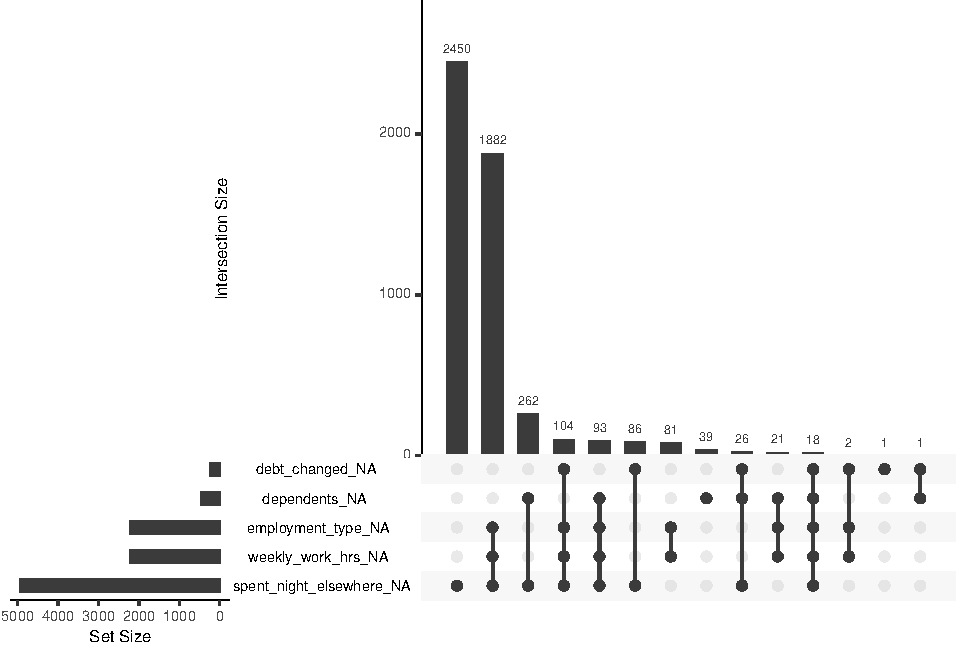
\includegraphics{final_phase2_report_files/figure-latex/unnamed-chunk-33-1} \end{center}

\begin{tabular}{l|r|r}
\hline
variable & n\_miss & pct\_miss\\
\hline
spent\_night\_elsewhere & 4921 & 95.0917874\\
\hline
employment\_type & 2201 & 42.5314010\\
\hline
weekly\_work\_hrs & 2201 & 42.5314010\\
\hline
dependents & 460 & 8.8888889\\
\hline
expenditures\_changed & 238 & 4.5990338\\
\hline
income\_changed & 238 & 4.5990338\\
\hline
fed\_aid\_changed & 238 & 4.5990338\\
\hline
debt\_changed & 238 & 4.5990338\\
\hline
FI\_q30 & 177 & 3.4202899\\
\hline
FI\_q31 & 177 & 3.4202899\\
\hline
FI\_q26 & 157 & 3.0338164\\
\hline
FI\_q27 & 157 & 3.0338164\\
\hline
FI\_q28 & 157 & 3.0338164\\
\hline
know\_homeless\_student & 115 & 2.2222222\\
\hline
federal\_student\_aid & 115 & 2.2222222\\
\hline
residence & 80 & 1.5458937\\
\hline
permanent\_address & 80 & 1.5458937\\
\hline
household\_head & 56 & 1.0821256\\
\hline
gender & 22 & 0.4251208\\
\hline
respondent\_id & 0 & 0.0000000\\
\hline
enrollment & 0 & 0.0000000\\
\hline
employment & 0 & 0.0000000\\
\hline
ethnicity & 0 & 0.0000000\\
\hline
total\_income & 0 & 0.0000000\\
\hline
academic\_level & 0 & 0.0000000\\
\hline
college/school & 0 & 0.0000000\\
\hline
mode\_transport & 0 & 0.0000000\\
\hline
transport\_reliability & 0 & 0.0000000\\
\hline
living\_alone & 0 & 0.0000000\\
\hline
\end{tabular}

\begin{center}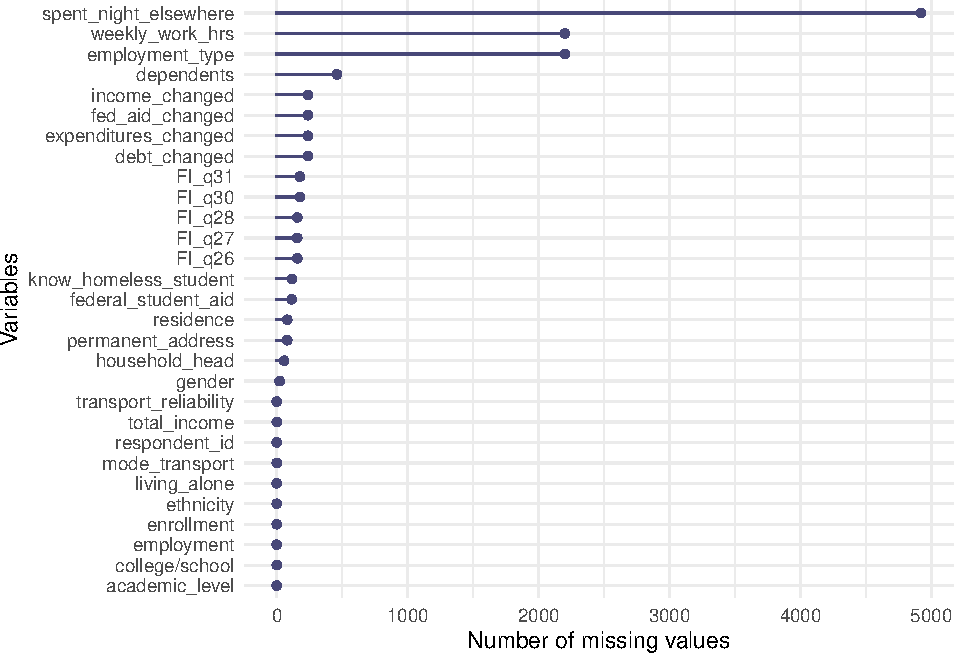
\includegraphics{final_phase2_report_files/figure-latex/unnamed-chunk-33-2} \end{center}

\begin{center}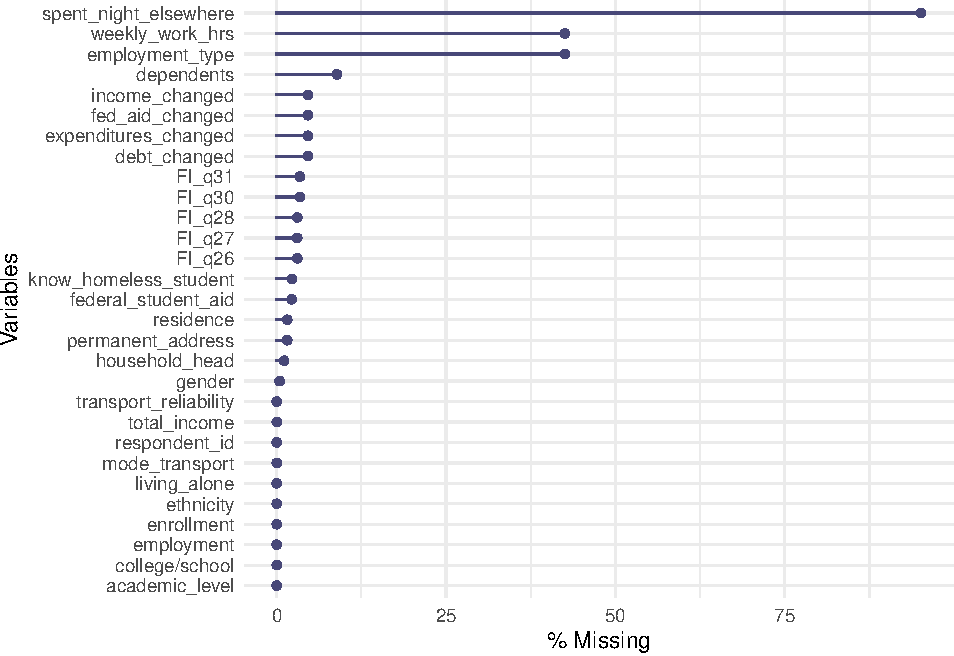
\includegraphics{final_phase2_report_files/figure-latex/unnamed-chunk-33-3} \end{center}

\hypertarget{codes}{%
\subsection{Codes}\label{codes}}

Codes for the analysis is available via a github repository upon request.

\newpage{}

\end{document}
